\documentclass[10pt]{article}

\usepackage[a4paper,margin=0.65in]{geometry}
\usepackage{amsmath,amssymb}
\usepackage{graphicx}
\usepackage{booktabs}
\usepackage{array}
\usepackage{float}
\usepackage{hyperref}
\usepackage{enumitem}
\usepackage{xcolor}
\usepackage{tikz}
\usetikzlibrary{positioning,arrows.meta,shapes.geometric,fit,calc}

\setlist{nosep,leftmargin=*}
\renewcommand{\arraystretch}{1.2}
\setlength{\parindent}{0pt}
\setlength{\parskip}{2pt}

\tikzset{
layer/.style={
draw,
rounded corners,
minimum width=1.7cm,
minimum height=0.65cm,
align=center,
fill=blue!10,
font=\scriptsize
},
smalllayer/.style={
draw,
rounded corners,
minimum width=1.35cm,
minimum height=0.58cm,
align=center,
fill=green!10,
font=\scriptsize
},
arrow/.style={
-{Latex[length=2mm]},
thin
}
}

\begin{document}

%%%%%%%%%%%%%%%%%%%%%%%%%%%%%%%%%%%%%%%%%%%%%%%%%%%%%%%%%%%%
% TITLE
%%%%%%%%%%%%%%%%%%%%%%%%%%%%%%%%%%%%%%%%%%%%%%%%%%%%%%%%%%%%

\begin{center}

{\large\textbf{Shiv Nadar University Chennai}}

\vspace{2mm}

{\normalsize\textbf{CS3807 -- Deep Learning Laboratory}}

\vspace{2mm}

{\large\textbf{Experiment 7}}

\vspace{1mm}

{\normalsize\textbf{End-to-End Study of Autoencoders, Convolutional}}

{\normalsize\textbf{Autoencoders, Denoising Autoencoders and Variational Autoencoders}}

\end{center}

\vspace{3mm}

\begin{tabular}{|p{3.4cm}|p{9.0cm}|p{1.4cm}|}
\hline
Degree \& Branch &
B.Tech Artificial Intelligence \& Data Science &
Semester V\\
\hline
Subject Code \& Name &
CS3807 -- Deep Learning Laboratory &
AY: 2026--27\\
\hline
\end{tabular}

%%%%%%%%%%%%%%%%%%%%%%%%%%%%%%%%%%%%%%%%%%%%%%%%%%%%%%%%%%%%
\section*{1. Objective}

The objective of this experiment is to develop an end-to-end understanding of
autoencoders and their variants for image representation, reconstruction,
denoising and generative modeling.

The experiment begins with a fully connected autoencoder, progresses to a
Convolutional Autoencoder (CAE), introduces image corruption for denoising,
and finally develops a Variational Autoencoder (VAE). Students will visualize
the learned latent representation, compare reconstruction quality using
quantitative and qualitative measures, and explore the generative capability
of the VAE.

The same image dataset and a controlled experimental protocol should be used
throughout the experiment wherever possible.

%%%%%%%%%%%%%%%%%%%%%%%%%%%%%%%%%%%%%%%%%%%%%%%%%%%%%%%%%%%%
\section*{2. Learning Outcomes}

After completing this experiment, students will be able to:

\begin{itemize}
\item explain the encoder--latent--decoder structure of an autoencoder;
\item prepare image data for reconstruction-based learning;
\item implement a fully connected autoencoder;
\item implement a Convolutional Autoencoder for image reconstruction;
\item introduce controlled noise and build a denoising autoencoder;
\item evaluate reconstruction using MSE, MAE and SSIM;
\item visualize and interpret latent representations;
\item explain the probabilistic latent representation of a VAE;
\item implement the reparameterization trick;
\item calculate and interpret reconstruction and KL-divergence losses;
\item generate new images by sampling from a learned latent space; and
\item compare deterministic and variational latent representations.
\end{itemize}

%%%%%%%%%%%%%%%%%%%%%%%%%%%%%%%%%%%%%%%%%%%%%%%%%%%%%%%%%%%%
\section*{3. Dataset and Experimental Setup}

\textbf{Dataset: MNIST Handwritten Digit Dataset}

MNIST contains grayscale images of handwritten digits from 0 to 9. Each image
has spatial dimensions

\[
28\times28\times1.
\]

The dataset was loaded directly using Keras/TensorFlow:

\url{https://www.tensorflow.org/api_docs/python/tf/keras/datasets/mnist}

\textbf{Laboratory subset used:} A stratified subset of 10,000 training
images and 2,000 test images (seed = 42) was used for all experiments.
Pixel values were normalized from $[0,255]$ to $[0,1]$.

\begin{center}
\begin{tabular}{|c|c|}
\hline
Digit & Training Count\\
\hline
0 & 987\\
1 & 1{,}124\\
2 & 993\\
3 & 1{,}022\\
4 & 974\\
5 & 904\\
6 & 986\\
7 & 1{,}044\\
8 & 975\\
9 & 991\\
\hline
\end{tabular}
\end{center}

The stratified sampling keeps all ten classes close to balanced
($\approx900$--$1{,}124$ images each out of 10,000).

The labels are not required as reconstruction targets. The original image is
the target:

\[
\boxed{x\rightarrow \text{Encoder}\rightarrow z
\rightarrow\text{Decoder}\rightarrow\hat{x}}
\]

where $x$ is the input image and $\hat{x}$ is its reconstruction.

%%%%%%%%%%%%%%%%%%%%%%%%%%%%%%%%%%%%%%%%%%%%%%%%%%%%%%%%%%%%
\section*{4. Source Code}

The complete implementation (fully connected autoencoder, convolutional
autoencoder, denoising convolutional autoencoder, variational autoencoder,
and all reconstruction/latent-space analyses) is available at the following
GitHub repository:

\begin{center}
\url{https://github.com/PolarFox08/Deep-Learning-Lab/tree/main/Deep%20Learning%20Lab%207}
\end{center}

%%%%%%%%%%%%%%%%%%%%%%%%%%%%%%%%%%%%%%%%%%%%%%%%%%%%%%%%%%%%
\section*{5. Expected Input and Output}

\subsection*{Expected Input}

Each input image has shape

\[
28\times28\times1.
\]

For a batch of 32 images:

\[
X\in\mathbb{R}^{32\times28\times28\times1}.
\]

Pixel values should be converted from

\[
[0,255]\rightarrow[0,1].
\]

For a fully connected autoencoder, the image may be flattened:

\[
28\times28=784.
\]

Therefore,

\[
x\in\mathbb{R}^{784}.
\]

For a convolutional autoencoder, retain the spatial structure:

\[
x\in\mathbb{R}^{28\times28\times1}.
\]

\subsection*{Expected Output}

The primary output is a reconstructed image:

\[
\hat{x}\in\mathbb{R}^{28\times28\times1}.
\]

Students must display:

\begin{verbatim}
Original image
Reconstructed image
Reconstruction error
\end{verbatim}

For the denoising model, display:

\begin{verbatim}
Original clean image
Noisy image
Denoised reconstruction
\end{verbatim}

For the VAE, display newly generated samples obtained by sampling from the
latent distribution.

%%%%%%%%%%%%%%%%%%%%%%%%%%%%%%%%%%%%%%%%%%%%%%%%%%%%%%%%%%%%
\section*{6. Overall Experimental Pipeline}

The complete experiment follows:

\begin{center}
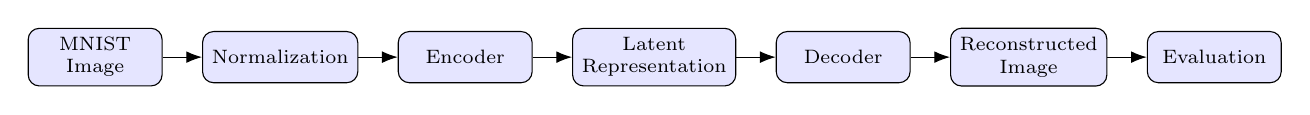
\begin{tikzpicture}[node distance=5mm]
\node[layer](a){MNIST\\Image};
\node[layer,right=of a](b){Normalization};
\node[layer,right=of b](c){Encoder};
\node[layer,right=of c](d){Latent\\Representation};
\node[layer,right=of d](e){Decoder};
\node[layer,right=of e](f){Reconstructed\\Image};
\node[layer,right=of f](g){Evaluation};

\foreach \x/\y in {a/b,b/c,c/d,d/e,e/f,f/g}
\draw[arrow](\x)--(\y);
\end{tikzpicture}
\end{center}

The experiment consists of four related studies:

\begin{enumerate}
\item Fully Connected Autoencoder
\item Convolutional Autoencoder
\item Denoising Convolutional Autoencoder
\item Variational Autoencoder
\end{enumerate}

%%%%%%%%%%%%%%%%%%%%%%%%%%%%%%%%%%%%%%%%%%%%%%%%%%%%%%%%%%%%
\section*{7. Exploring Autoencoders}

An autoencoder learns to reproduce its input at the output.

The encoder maps the input to a lower-dimensional representation:

\[
z=f_{\theta}(x),
\]

and the decoder reconstructs the input:

\[
\hat{x}=g_{\phi}(z).
\]

The training objective is to minimize reconstruction error:

\[
\mathcal{L}_{rec}
=
\frac{1}{N}\sum_{i=1}^{N}
\|x_i-\hat{x}_i\|^2.
\]

\begin{center}
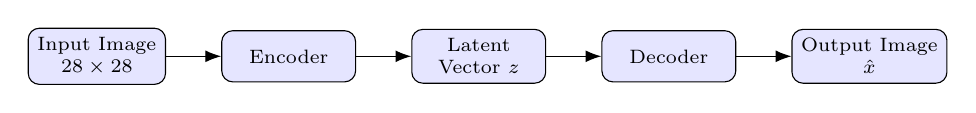
\begin{tikzpicture}[node distance=7mm]
\node[layer](a){Input Image\\$28\times28$};
\node[layer,right=of a](b){Encoder};
\node[layer,right=of b](c){Latent\\Vector $z$};
\node[layer,right=of c](d){Decoder};
\node[layer,right=of d](e){Output Image\\$\hat{x}$};

\foreach \x/\y in {a/b,b/c,c/d,d/e}
\draw[arrow](\x)--(\y);
\end{tikzpicture}
\end{center}

The latent vector is a compressed representation of the input.

%%%%%%%%%%%%%%%%%%%%%%%%%%%%%%%%%%%%%%%%%%%%%%%%%%%%%%%%%%%%
\section*{8. Fully Connected Autoencoder}

Flatten each image from

\[
28\times28=784
\]

to a vector of length 784.

Architecture used (matches the suggested configuration exactly):

\begin{center}
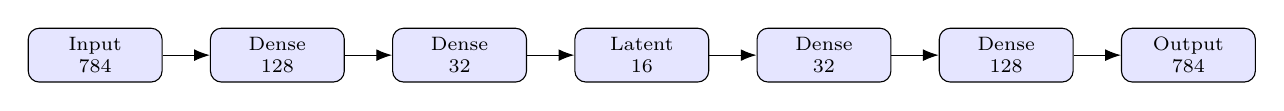
\begin{tikzpicture}[node distance=6mm]
\node[layer](a){Input\\784};
\node[layer,right=of a](b){Dense\\128};
\node[layer,right=of b](c){Dense\\32};
\node[layer,right=of c](d){Latent\\16};
\node[layer,right=of d](e){Dense\\32};
\node[layer,right=of e](f){Dense\\128};
\node[layer,right=of f](g){Output\\784};

\foreach \x/\y in {a/b,b/c,c/d,d/e,e/f,f/g}
\draw[arrow](\x)--(\y);
\end{tikzpicture}
\end{center}

ReLU activation was used in hidden layers and sigmoid activation in the output
layer.

\textbf{Configuration used:}

\begin{center}
\begin{tabular}{|l|l|}
\hline
Parameter & Value\\
\hline
Latent dimension & 16\\
Optimizer & Adam\\
Learning rate & $10^{-3}$\\
Batch size & 128\\
Epochs & 20\\
Loss & Binary Cross-Entropy\\
Total parameters & 211{,}040\\
\hline
\end{tabular}
\end{center}

%%%%%%%%%%%%%%%%%%%%%%%%%%%%%%%%%%%%%%%%%%%%%%%%%%%%%%%%%%%%
\section*{9. Required Analysis of the Basic Autoencoder}

\textbf{Plot 1: Original versus Reconstructed Images}

\begin{center}
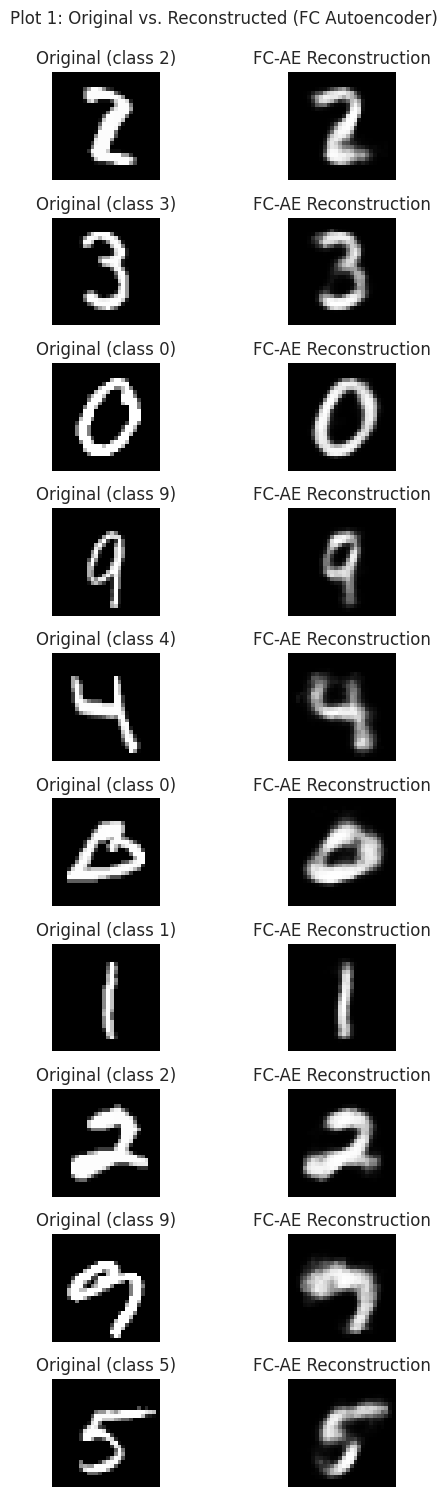
\includegraphics[width=0.4\textwidth]{plots/plot1_orig_recon_fc.png}
\end{center}

\textbf{Inference :} All the digits were reconstructed and are legible to read, but noticeably blurrier compared to the input. Simple straight stroked-digits like 1 and 4 and simple curves like 0 are reconstructed more sharper, but slightly complex digits like 9 and 5 are less clear and more blurry. This is consistent with a fully connected network having to reconstruct every pixel independently from a 16-dimensional bottleneck with no explicit notion of spatial locality.

\textbf{Plot 2: Training and Validation Reconstruction Loss}

\begin{center}
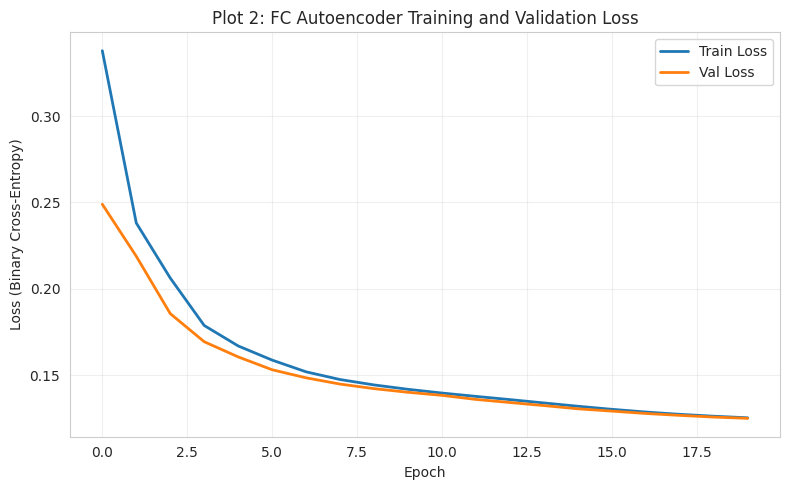
\includegraphics[width=0.55\textwidth]{plots/plot2_fc_loss.png}
\end{center}

\textbf{Required inference:} Both curves look similar and converge at a similar value too. This is expected as the dataset is the same MNIST and hence no drift in distribution or anything else. No evidence of overfitting found too.

%%%%%%%%%%%%%%%%%%%%%%%%%%%%%%%%%%%%%%%%%%%%%%%%%%%%%%%%%%%%
\section*{10. Reconstruction Metrics}

Students must calculate the following metrics on the test set.

\subsection*{Mean Squared Error}

\[
MSE=
\frac{1}{N}
\sum_{i=1}^{N}
(x_i-\hat{x}_i)^2.
\]

\subsection*{Mean Absolute Error}

\[
MAE=
\frac{1}{N}
\sum_{i=1}^{N}
|x_i-\hat{x}_i|.
\]

\subsection*{Structural Similarity}

Calculate SSIM between the original and reconstructed images.

The implementation may use:

\url{https://scikit-image.org/docs/stable/api/skimage.metrics.html}

\begin{center}
\begin{tabular}{|l|c|}
\hline
Metric & Value\\
\hline
Test MSE & 0.021037\\
Test MAE & 0.056284\\
Mean SSIM & 0.7621\\
\hline
\end{tabular}
\end{center}

%%%%%%%%%%%%%%%%%%%%%%%%%%%%%%%%%%%%%%%%%%%%%%%%%%%%%%%%%%%%
\section*{11. Convolutional Autoencoder}

A Convolutional Autoencoder preserves spatial structure and uses convolutional
operations in the encoder and upsampling operations in the decoder.

The implementation used:

\begin{verbatim}
Input(28,28,1)
Conv2D(32, 3, activation='relu', padding='same')
MaxPooling2D(2, padding='same')
Conv2D(64, 3, activation='relu', padding='same')
MaxPooling2D(2, padding='same')
Conv2D(64, 3, activation='relu', padding='same')
UpSampling2D(2)
Conv2D(32, 3, activation='relu', padding='same')
UpSampling2D(2)
Conv2D(1, 3, activation='sigmoid', padding='same')
\end{verbatim}

(UpSampling2D was used rather than Conv2DTranspose; see Section 30, Exercise 4
for the untested transposed-convolution variant.) Same optimizer/loss/batch
size/epochs as the FC autoencoder (Adam, lr $=10^{-3}$, BCE, batch 128, 20
epochs). Total parameters: 74{,}497.

%%%%%%%%%%%%%%%%%%%%%%%%%%%%%%%%%%%%%%%%%%%%%%%%%%%%%%%%%%%%
\section*{12. Comparing Fully Connected and Convolutional Autoencoders}

Both models were trained using the same training and test images.

\begin{center}
\begin{tabular}{|l|c|c|c|c|}
\hline
Model & MSE & MAE & SSIM & Parameters\\
\hline
Fully Connected AE & 0.021037 & 0.056284 & 0.7621 & 211{,}040\\
Convolutional AE   & 0.002561 & 0.015044 & 0.9746 & 74{,}497\\
\hline
\end{tabular}
\end{center}

\textbf{Plot 3: Reconstruction Comparison}

\begin{center}
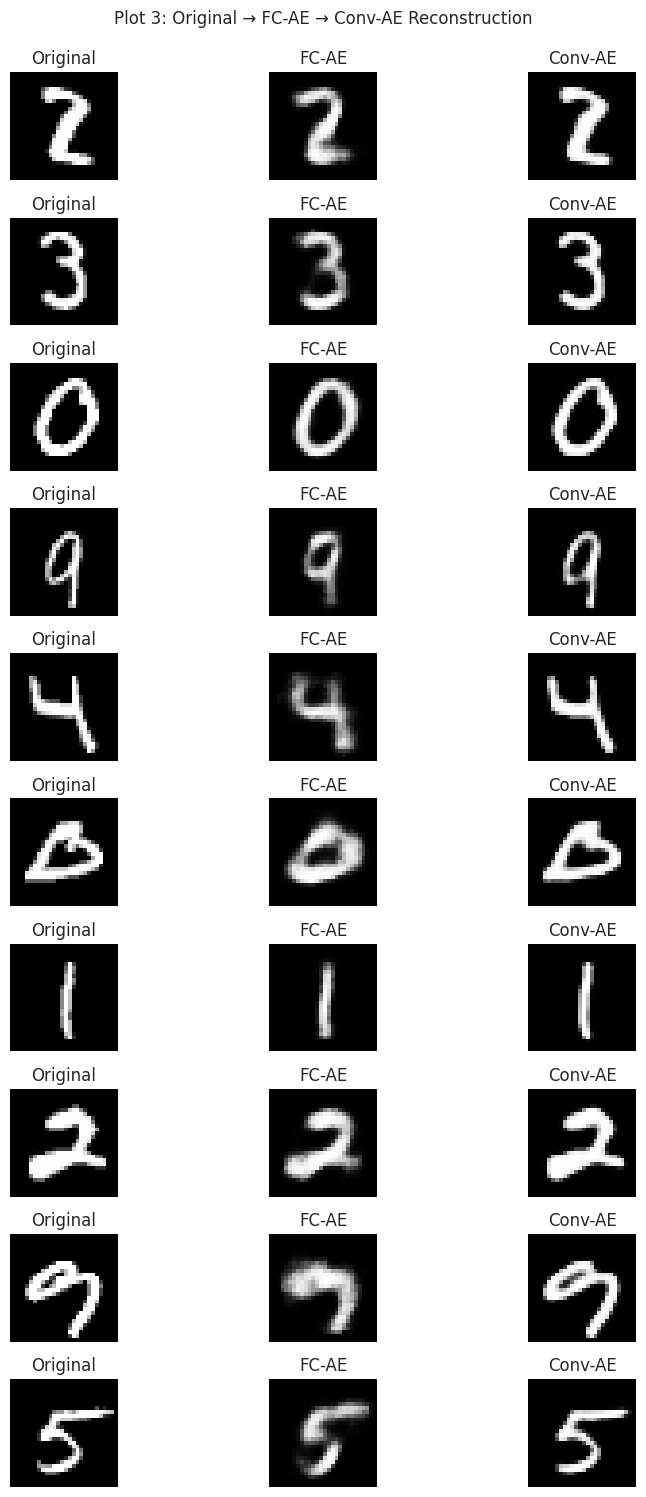
\includegraphics[width=0.55\textwidth]{plots/plot3_fc_conv.png}
\end{center}

\textbf{Required inference :} Even with less paramters Conv-AE images are much more sharper and closer to the original images compared to FC-AE. This is because spatial property is preserved through convolution as each pixel gets a value based on its neighborhood pixels rather than a flattened bottleneck. Curly images (9,5,3) are very sharp and their curves and holes are more defined and closer to actual, thanks to convoultion's spatial property.

%%%%%%%%%%%%%%%%%%%%%%%%%%%%%%%%%%%%%%%%%%%%%%%%%%%%%%%%%%%%
\section*{13. Denoising Autoencoder}

A denoising autoencoder receives a corrupted image but is trained to
reconstruct the original clean image.

The training mapping is:

\[
\boxed{\tilde{x}\rightarrow\text{Encoder}\rightarrow z
\rightarrow\text{Decoder}\rightarrow\hat{x}}
\]

where $\tilde{x}$ is a noisy version of the clean image $x$. The same
Conv-AE architecture as Section 11 was reused for the denoising model
(74{,}497 parameters), trained with noisy input $\rightarrow$ clean target,
using Gaussian noise at $\sigma=0.2$ as the main training noise level.

\begin{center}
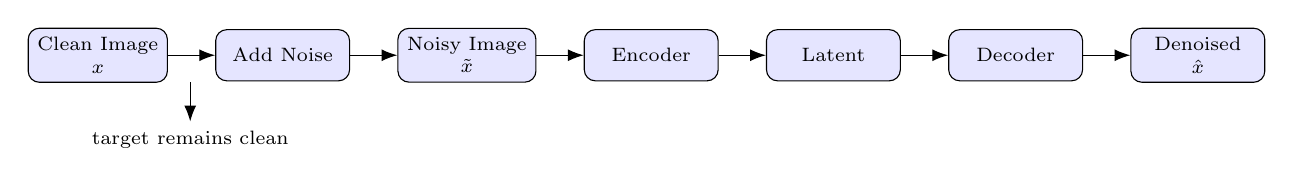
\begin{tikzpicture}[node distance=6mm]
\node[layer](a){Clean Image\\$x$};
\node[layer,right=of a](b){Add Noise};
\node[layer,right=of b](c){Noisy Image\\$\tilde{x}$};
\node[layer,right=of c](d){Encoder};
\node[layer,right=of d](e){Latent};
\node[layer,right=of e](f){Decoder};
\node[layer,right=of f](g){Denoised\\$\hat{x}$};

\foreach \x/\y in {a/b,b/c,c/d,d/e,e/f,f/g}
\draw[arrow](\x)--(\y);

\draw[arrow]($(a.south)!0.5!(b.south)$) -- ++(0,-5mm)
node[below,font=\scriptsize]{target remains clean};
\end{tikzpicture}
\end{center}

%%%%%%%%%%%%%%%%%%%%%%%%%%%%%%%%%%%%%%%%%%%%%%%%%%%%%%%%%%%%
\section*{14. Adding Image Noise}

\subsection*{Gaussian Noise (implemented and evaluated)}

\[
\tilde{x}=x+n,
\qquad
n\sim\mathcal{N}(0,\sigma^2).
\]

Standard deviations used:

\[
\sigma\in\{0.1,0.2,0.3\},
\]

clipped to $[0,1]$. The denoising model was trained once, at
$\sigma=0.2$, and evaluated against noisy test images at all three levels.

\subsection*{Salt-and-Pepper Noise (implemented but not evaluated)}

A salt-and-pepper corruption function was implemented in the notebook
(randomly replacing a proportion of pixels with 0 or 1), but no
salt-and-pepper denoising model was actually trained or evaluated in this
run -- see Section 30, Exercise 2.

%%%%%%%%%%%%%%%%%%%%%%%%%%%%%%%%%%%%%%%%%%%%%%%%%%%%%%%%%%%%
\section*{15. Required Denoising Plots}

\textbf{Plot 4: Clean vs. Noisy vs. Denoised}

\begin{center}
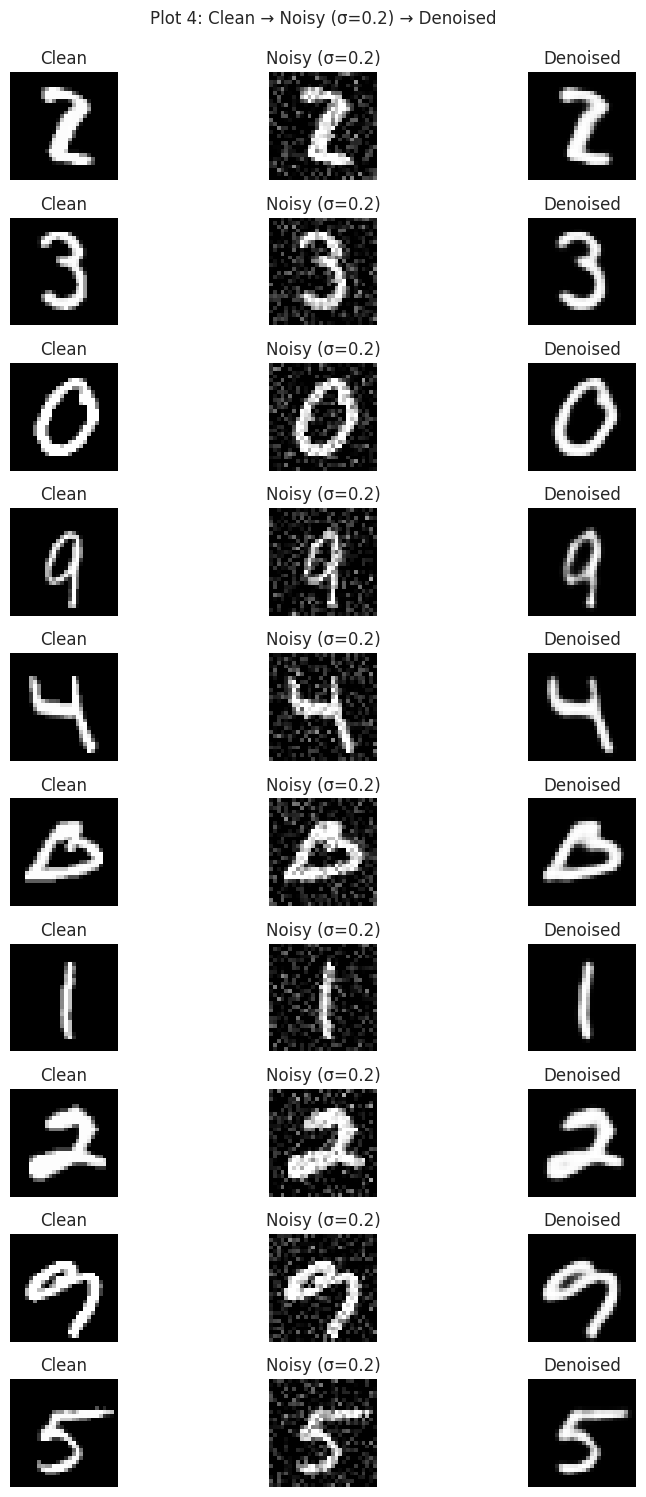
\includegraphics[width=0.55\textwidth]{plots/plot4_denoise.png}
\end{center}

\textbf{Inference :} At $\sigma=0.2$, the input images gets heavily mixed with random extreme pixels making some of the strokes look illegible. However the AE is able to learn the natural strokes and produce an almost similar copy of the actual numbers, with very mild variations

\textbf{Plot 5: Noise Level vs. Reconstruction Quality}

\begin{center}
\begin{tabular}{|c|c|c|c|}
\hline
Noise Level ($\sigma$) & MSE & MAE & SSIM\\
\hline
0.1 & 0.003471 & 0.017457 & 0.9608\\
0.2 & 0.004465 & 0.020965 & 0.9475\\
0.3 & 0.006812 & 0.028429 & 0.8945\\
\hline
\end{tabular}
\end{center}

\begin{center}
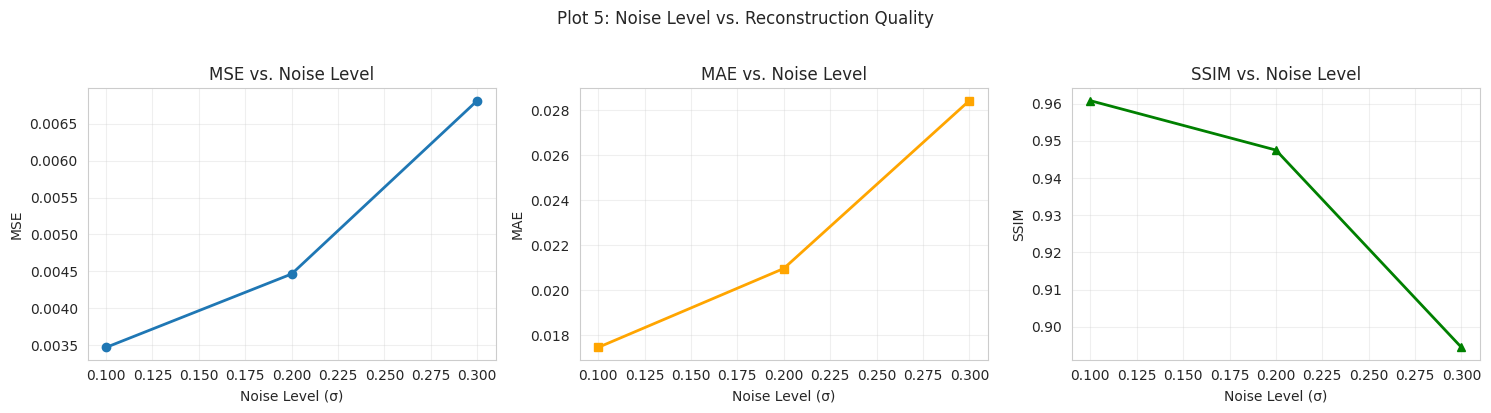
\includegraphics[width=0.85\textwidth]{plots/plot5_noise_quality.png}
\end{center}

\textbf{Required inference:} MSE and MAE loss rise roughly linearly while SSIM decreases linearly as noise increases
from $\sigma=0.1$ to $0.3$. This is the expected output as the more a number a gets corrupter the more the loss will be while the structural similarity decreases.  The error at max noise is still very less and the model would be able to figure out the natural strokes and denoise the numbers easily.

%%%%%%%%%%%%%%%%%%%%%%%%%%%%%%%%%%%%%%%%%%%%%%%%%%%%%%%%%%%%
\section*{16. Variational Autoencoder}

A conventional autoencoder maps an input to a deterministic latent vector:

\[
z=f(x).
\]

A VAE instead learns a probability distribution:

\[
q_{\phi}(z|x)
=
\mathcal{N}
\left(
\mu(x),
\operatorname{diag}(\sigma^2(x))
\right).
\]

The encoder produces:

\[
\mu,\qquad \log\sigma^2.
\]

A latent vector is sampled using the reparameterization trick:

\[
z=\mu+\sigma\odot\epsilon,
\qquad
\epsilon\sim\mathcal{N}(0,I).
\]

\begin{center}
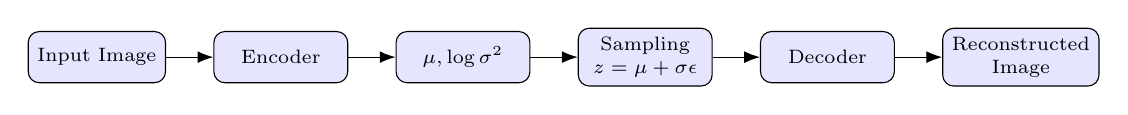
\begin{tikzpicture}[node distance=6mm]
\node[layer](a){Input Image};
\node[layer,right=of a](b){Encoder};
\node[layer,right=of b](c){$\mu,\log\sigma^2$};
\node[layer,right=of c](d){Sampling\\$z=\mu+\sigma\epsilon$};
\node[layer,right=of d](e){Decoder};
\node[layer,right=of e](f){Reconstructed\\Image};

\foreach \x/\y in {a/b,b/c,c/d,d/e,e/f}
\draw[arrow](\x)--(\y);
\end{tikzpicture}
\end{center}

%%%%%%%%%%%%%%%%%%%%%%%%%%%%%%%%%%%%%%%%%%%%%%%%%%%%%%%%%%%%
\section*{17. VAE Loss Function}

The VAE objective consists of two components.

\subsection*{Reconstruction Loss}

\[
\mathcal{L}_{rec}
=
-\mathbb{E}_{q_{\phi}(z|x)}
[\log p_{\theta}(x|z)].
\]

Binary cross-entropy was used, scaled by $28\times28$ (summed rather than
averaged over pixels) to balance it against the KL term.

\subsection*{KL Divergence}

\[
D_{KL}
\left(
q_{\phi}(z|x)\parallel p(z)
\right)
=
-\frac{1}{2}
\sum_j
\left(
1+\log\sigma_j^2-\mu_j^2-\sigma_j^2
\right).
\]

The total loss is

\[
\boxed{
\mathcal{L}_{VAE}
=
\mathcal{L}_{rec}
+
\mathcal{L}_{KL}
}
\]

where the prior is

\[
p(z)=\mathcal{N}(0,I).
\]

\textbf{Training configuration used:} Adam, lr $=10^{-3}$, batch size 128,
30 epochs, trained on the 10,000-image training set with \textbf{no
held-out validation split} (\texttt{vae.fit} was called without
\texttt{validation\_data}).

\begin{center}
\begin{tabular}{|l|c|c|}
\hline
Epoch & Reconstruction Loss & KL Loss\\
\hline
1 (first)  & 191.63 & 2.62\\
30 (final) & 140.65 & 3.55\\
\hline
\end{tabular}
\end{center}

Total loss fell from 194.26 (epoch 1) to 144.19 (epoch 30). Reconstruction
loss dropped substantially and monotonically over training, while KL loss
rose only slightly (2.62 $\rightarrow$ 3.55) and stayed small relative to
the reconstruction term -- the model prioritized fitting the data while
keeping the latent distribution only mildly regularized toward the prior.

%%%%%%%%%%%%%%%%%%%%%%%%%%%%%%%%%%%%%%%%%%%%%%%%%%%%%%%%%%%%
\section*{18. VAE Implementation}

A small, 2-dimensional latent space was used so that it can be visualized:

\[
z\in\mathbb{R}^{2}.
\]

The encoder produces:

\[
\mu\in\mathbb{R}^{2},
\qquad
\log\sigma^2\in\mathbb{R}^{2}.
\]

The implemented architecture was:

\begin{center}
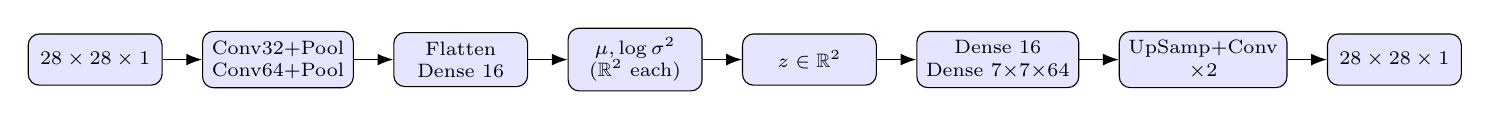
\begin{tikzpicture}[node distance=5mm]
\node[layer](a){$28\times28\times1$};
\node[layer,right=of a](b){Conv32+Pool\\Conv64+Pool};
\node[layer,right=of b](c){Flatten\\Dense 16};
\node[layer,right=of c](d){$\mu,\log\sigma^2$\\($\mathbb{R}^2$ each)};
\node[layer,right=of d](e){$z\in\mathbb{R}^2$};
\node[layer,right=of e](f){Dense 16\\Dense $7{\times}7{\times}64$};
\node[layer,right=of f](g){UpSamp+Conv\\$\times2$};
\node[layer,right=of g](h){$28\times28\times1$};

\foreach \x/\y in {a/b,b/c,c/d,d/e,e/f,f/g,g/h}
\draw[arrow](\x)--(\y);
\end{tikzpicture}
\end{center}

Total trainable parameters: 70{,}594.

%%%%%%%%%%%%%%%%%%%%%%%%%%%%%%%%%%%%%%%%%%%%%%%%%%%%%%%%%%%%
\section*{19. Exploring the VAE Latent Space}

Since the latent dimension is two, the encoded test images can be visualized
in a two-dimensional plane.

\textbf{Plot 6: VAE Latent Space}

\begin{center}
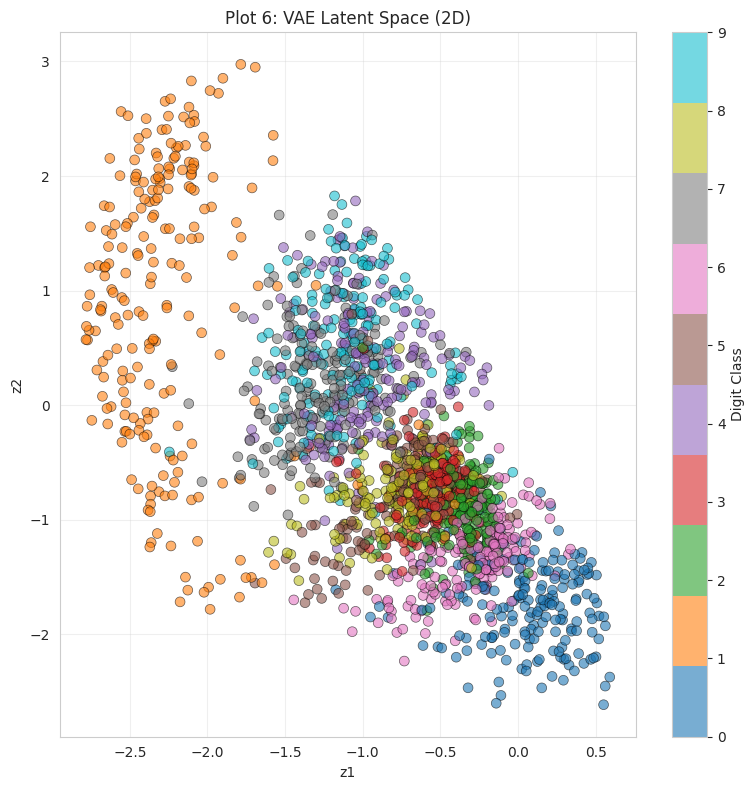
\includegraphics[width=0.5\textwidth]{plots/plot6_latent_space.png}
\end{center}

\textbf{Required inference :} Digits 1 and 0 form visually separating clusters. Other digits like 3,8 and 7,9,4 form heavily overlapping regions. This indicates the 2 dimensional bottleneck is not enough to linearly separate all 10 digits without overlaps (even though points of a specific digit form tight regions) 

%%%%%%%%%%%%%%%%%%%%%%%%%%%%%%%%%%%%%%%%%%%%%%%%%%%%%%%%%%%%
\section*{20. Generating New Images with the VAE}

Sample points from

\[
z\sim\mathcal{N}(0,I).
\]

Pass the sampled latent vectors through the decoder.

\textbf{Plot 7: Randomly Generated Images}

\begin{center}
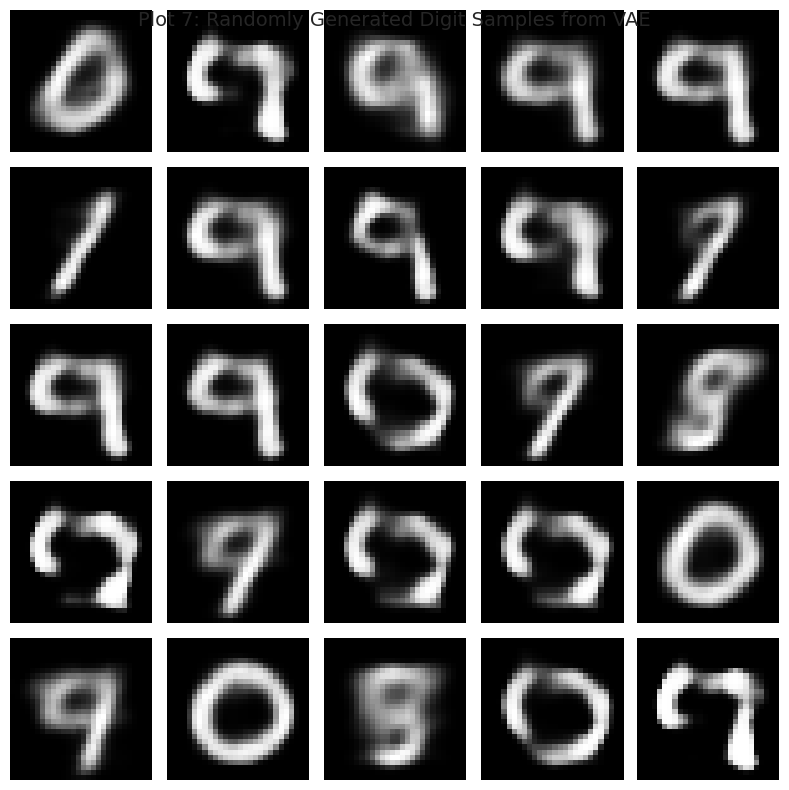
\includegraphics[width=0.45\textwidth]{plots/plot7_generated.png}
\end{center}

\textbf{Inference :} The generated digits are recognizable but have a very small diversity in them with mostly digits like 9,8 and 0s generated most of the time. This is because the mean of the latent space distribution is filled with overlaps of these numbers (3,8,6,7,9) so the generated data also resembles these digits (circles and a flat line). This low-diverse sampling can be seen as a disadvantage of VAEs.

%%%%%%%%%%%%%%%%%%%%%%%%%%%%%%%%%%%%%%%%%%%%%%%%%%%%%%%%%%%%
\section*{21. Latent Space Interpolation}

Select two latent vectors:

\[
z_A,\qquad z_B.
\]

Construct

\[
z(\alpha)=(1-\alpha)z_A+\alpha z_B,
\qquad
\alpha\in[0,1].
\]

11 values were used ($\alpha=0,0.1,\ldots,1.0$), interpolating between the
encoded means of a test digit \textbf{0} ($z_A$) and a test digit
\textbf{9} ($z_B$).

\textbf{Plot 8: Latent Space Interpolation}

\begin{center}
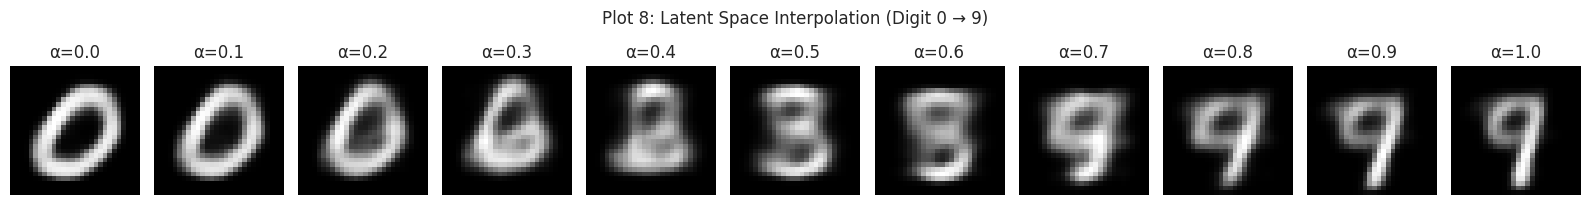
\includegraphics[width=0.9\textwidth]{plots/plot8_interp.png}
\end{center}

\textbf{Required inference :} The decoded
image changes smoothly and continuously along the path: a clean 0
($\alpha=0$--$0.2$) gradually closes and tilts into a 6-like shape ($\alpha\approx0.3$--$0.5$), then thickens into an 8-like/ambiguous shape ($\alpha\approx0.6$), before opening into a clear 9 ($\alpha\approx0.7$-- $1.0$). There are no abrupt jumps or unrecognizable/broken intermediate frames anywhere along the path, confirming the learned latent space is
locally continuous and semantically meaningful in this region, not just a lookup table of memorized points.

%%%%%%%%%%%%%%%%%%%%%%%%%%%%%%%%%%%%%%%%%%%%%%%%%%%%%%%%%%%%
\section*{22. Reconstruction Comparison Across Models}

\begin{center}
\begin{tabular}{|l|c|c|c|c|}
\hline
Model & MSE & MAE & SSIM & Parameters\\
\hline
Fully Connected AE & 0.021037 & 0.056284 & 0.7621 & 211{,}040\\
Convolutional AE   & 0.002561 & 0.015044 & 0.9746 & 74{,}497\\
Denoising CAE ($\sigma=0.2$) & 0.004465 & 0.020965 & 0.9475 & 74{,}497\\
\hline
\end{tabular}
\end{center}

For the VAE, its reconstruction loss is reported separately because its
total objective also contains the KL-divergence term.

\begin{center}
\begin{tabular}{|l|c|}
\hline
VAE Metric & Value\\
\hline
Reconstruction Loss (final epoch, BCE-based) & 140.65\\
KL Loss (final epoch) & 3.55\\
Total Loss (final epoch) & 144.19\\
Test MSE & 0.045464\\
Test MAE & 0.108695\\
Mean SSIM & 0.4865\\
\hline
\end{tabular}
\end{center}

The VAE's test-set MSE/MAE/SSIM are clearly worse than all three
deterministic autoencoders above -- expected, since (a) its latent space is
only 2-dimensional (a much tighter bottleneck than the FC-AE's 16 or the
Conv-AE's $7\times7\times64$ feature map) and (b) its loss trades off
reconstruction fidelity against the KL regularization term, rather than
optimizing reconstruction alone.

%%%%%%%%%%%%%%%%%%%%%%%%%%%%%%%%%%%%%%%%%%%%%%%%%%%%%%%%%%%%
\section*{23. Required Plots}

The final report contains the following plots:

\begin{enumerate}
\item Original image versus reconstructed image. (Section 9, Plot 1)
\item Training and validation loss for the basic autoencoder. (Section 9, Plot 2)
\item Fully connected AE versus convolutional AE reconstruction. (Section 12, Plot 3)
\item Clean versus noisy versus denoised images. (Section 15, Plot 4)
\item Noise level versus MSE/MAE/SSIM. (Section 15, Plot 5)
\item VAE latent-space visualization. (Section 19, Plot 6)
\item Randomly generated VAE images. (Section 20, Plot 7)
\item Latent-space interpolation. (Section 21, Plot 8)
\item Training/validation reconstruction loss for the VAE.
% \textbf{Not
% available in this run} -- see Section 17: \texttt{vae.fit} was called
% without a validation split, so only a training-loss curve exists (reported
% as epoch 1 vs.\ epoch 30 values in Section 17's table), and no plot of it
% was generated in the notebook.
\item Reconstruction-error distribution on the test set. (Section 24, Plot 9)
\end{enumerate}


%%%%%%%%%%%%%%%%%%%%%%%%%%%%%%%%%%%%%%%%%%%%%%%%%%%%%%%%%%%%
\section*{24. Reconstruction Error Distribution}

Calculate the per-image reconstruction error:

\[
e_i=
\frac{1}{D}
\sum_{j=1}^{D}
(x_{ij}-\hat{x}_{ij})^2.
\]

\textbf{Plot 9: Distribution of Reconstruction Errors} (computed for the
Convolutional Autoencoder, the best-performing deterministic model)

\begin{center}
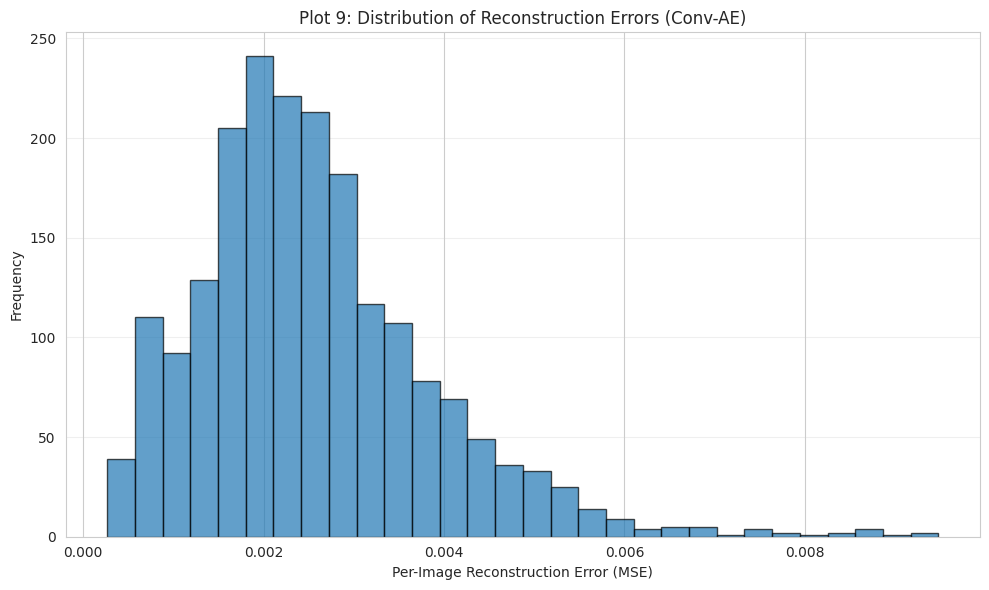
\includegraphics[width=0.65\textwidth]{plots/plot9_error_hist.png}
\end{center}

\textbf{Inference :} The the bulk of the 2,000 testimages have a per-image MSE between roughly 0.0015 and 0.003, with the distribution being heavilry right-skewed. So the typical reconstruction error is small and tightly clustered, but a minority of harder samples (the tail) drive up the mean MSE noticeably
above the mode.

%%%%%%%%%%%%%%%%%%%%%%%%%%%%%%%%%%%%%%%%%%%%%%%%%%%%%%%%%%%%
\section*{25. Required High-Error Image Analysis}

The five test images (Conv-AE) with the largest reconstruction errors:

\begin{center}
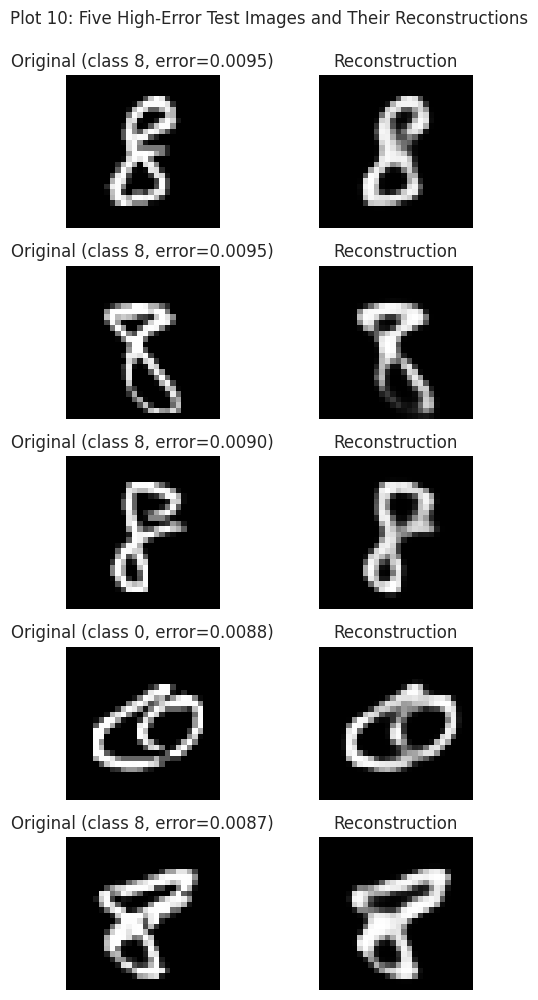
\includegraphics[width=0.4\textwidth]{plots/plot_higherror.png}
\end{center}

\begin{center}
\begin{tabular}{|c|c|c|}
\hline
Sample & True Class & Error (MSE) \\
\hline
1 & 8 & 0.0095 \\
2 & 8 & 0.0095 \\
3 & 8 & 0.0090 \\
4 & 0 & 0.0088 \\
5 & 8 & 0.0087 \\
\hline
\end{tabular}
\end{center}



\textbf{Explanation :} All of these images resembles an 8 somewhat. This implies the model find self- intersecting loops like 8 and looped 0 the most difficult. The reconstructed images are still recognizable but the details like the intersection area and the curves are blurry.

%%%%%%%%%%%%%%%%%%%%%%%%%%%%%%%%%%%%%%%%%%%%%%%%%%%%%%%%%%%%
\section*{26. Consolidated Results}

\begin{center}
\begin{tabular}{|l|c|c|c|c|}
\hline
Model & MSE & MAE & SSIM & Parameters \\
\hline
FC Autoencoder    & 0.021037 & 0.056284 & 0.7621 & 211{,}040 \\
Conv. Autoencoder & 0.002561 & 0.015044 & 0.9746 & 74{,}497  \\
Denoising CAE     & 0.004465 & 0.020965 & 0.9475 & 74{,}497  \\
VAE               & 0.045464 & 0.108695 & 0.4865 & 70{,}594  \\
\hline
\end{tabular}
\end{center}


%%%%%%%%%%%%%%%%%%%%%%%%%%%%%%%%%%%%%%%%%%%%%%%%%%%%%%%%%%%%
\section*{27. Required Inferences}

For every major plot, students must write a short inference containing:

\begin{enumerate}
\item What does the plot show?
\item What trend is observed?
\item Why might the observed trend occur?
\item What conclusion can be drawn?
\end{enumerate}

These are provided alongside each plot above (Sections 9, 12, 15, 19--21,
24--25). The following mandatory inferences are covered in the sections
indicated:

\begin{itemize}
\item effect of latent dimension on reconstruction -- Section 28;
\item difference between fully connected and convolutional reconstruction -- Section 12;
\item effect of Gaussian noise level -- Section 15 (Plot 5);
\item ability of the denoising autoencoder to recover image structure -- Section 15 (Plot 4);
\item characteristics of the VAE latent distribution -- Section 19;
\item structure of the two-dimensional VAE latent space -- Section 19;
\item quality and diversity of generated samples -- Section 20;
\item smoothness of latent-space interpolation -- Section 21;
\item relationship between reconstruction error and visual quality -- Sections 24--25;
\item differences between deterministic and probabilistic latent representations -- Section 22.
\end{itemize}

%%%%%%%%%%%%%%%%%%%%%%%%%%%%%%%%%%%%%%%%%%%%%%%%%%%%%%%%%%%%
\section*{28. Additional Latent-Dimension Study}

The basic (FC) autoencoder was retrained from scratch with:

\[
d_z\in\{2,8,16,32\}.
\]

\begin{center}
\begin{tabular}{|c|c|c|c|}
\hline
Latent Dimension & MSE & SSIM & Parameters\\
\hline
2  & 0.045616 & 0.4849 & 210{,}130\\
8  & 0.024291 & 0.7270 & 210{,}520\\
16 & 0.019654 & 0.7758 & 211{,}040\\
32 & 0.017896 & 0.7962 & 212{,}080\\
\hline
\end{tabular}
\end{center}

\textbf{Plot 10: Latent Dimension vs. Reconstruction MSE / SSIM}

\begin{center}
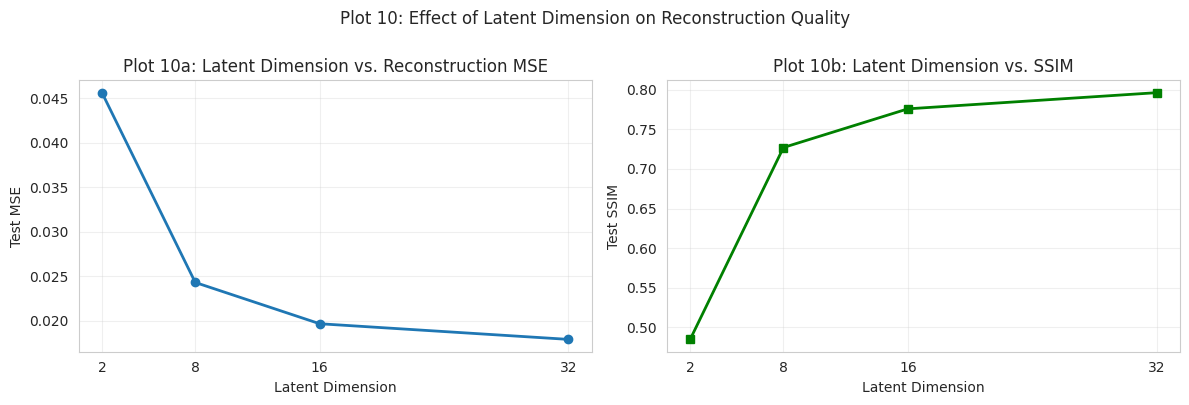
\includegraphics[width=0.85\textwidth]{plots/plot10_latentdim.png}
\end{center}

\textbf{Inference:} Both curves show significant gains initially as the latent dimension increases but at the 8-16 dim range the gain isnt that significant. This shows 2 dim is too restrictive but as dimension increases after a some point, the reconstruction quality becomes stable with  minimal performance gain.

%%%%%%%%%%%%%%%%%%%%%%%%%%%%%%%%%%%%%%%%%%%%%%%%%%%%%%%%%%%%
\section*{29. Discussion Questions}

\begin{enumerate}

\item \textbf{What is an autoencoder?} An autoencoder is a neural network
trained to reproduce its input at the output, learning a compressed
intermediate representation (latent code) in the process.

\item \textbf{What is the purpose of the encoder?} The encoder maps the
input to a lower-dimensional latent representation, compressing the input
while preserving essential information.

\item \textbf{What is the purpose of the decoder?} The decoder reconstructs
the original input from the latent code, translating the compressed
representation back to the original space.

\item \textbf{What is a latent representation?} A latent representation is
a compressed, lower-dimensional encoding of the input that captures its
essential features or structure.

\item \textbf{Why is the latent representation usually smaller than the
input?} A smaller latent dimension forces the autoencoder to learn a
compressed representation, acting as a bottleneck that removes noise and
irrelevant details.

\item \textbf{What happens when the latent dimension is too small?} The
model cannot capture enough information, resulting in high reconstruction
error and loss of fine details.

\item \textbf{What happens when the latent dimension is increased?}
Reconstruction quality improves, but the compression ratio decreases and
the model requires more parameters and computation.

\item \textbf{Why can a convolutional autoencoder preserve spatial
information more effectively?} Convolutional layers operate locally on
spatial neighborhoods, preserving local structure and relationships
between nearby pixels that fully connected layers lose.

\item \textbf{Differentiate an autoencoder and a denoising autoencoder.} A
standard autoencoder maps clean input to clean output. A denoising
autoencoder maps corrupted (noisy) input to clean output, learning to
remove noise.

\item \textbf{Why is the clean image used as the target in denoising?}
Using clean targets trains the model to reconstruct the original signal,
effectively learning to separate signal from noise.

\item \textbf{What happens when the noise level is increased?}
Reconstruction quality degrades, as the model must recover more severely
corrupted information; MSE increases and SSIM decreases.

\item \textbf{Why are MSE, MAE and SSIM useful for image reconstruction?}
MSE measures pixel-level error; MAE is robust to outliers; SSIM captures
perceived visual quality and structural similarity.

\item \textbf{What is a Variational Autoencoder?} A VAE learns a
probabilistic latent distribution, enabling both reconstruction and
generation of new samples by sampling from the learned distribution.

\item \textbf{How does a VAE differ from a conventional autoencoder?} A VAE
maps inputs to a probability distribution ($\mu,\sigma$) rather than a
point; samples are drawn using the reparameterization trick, enabling
smooth latent space interpolation.

\item \textbf{Why does a VAE learn a distribution instead of a single
latent vector?} A distribution enables smooth interpolation and
generation, making the latent space continuous and enabling meaningful
sample synthesis.

\item \textbf{What is the reparameterization trick?} It reformulates
$z=\mu+\sigma\odot\epsilon$ to enable backpropagation through the sampling
operation by separating the deterministic and stochastic components.

\item \textbf{Why is $\epsilon$ sampled from a standard normal
distribution?} The standard normal provides a universal source of
randomness that is transformed by $\mu$ and $\sigma$ to produce samples
from the desired distribution.

\item \textbf{What is the role of KL divergence in the VAE loss?} KL
divergence regularizes the latent distribution to match a standard normal
prior, ensuring a smooth, continuous latent space suitable for generation.

\item \textbf{What is the prior distribution used in the VAE?} The
standard normal distribution $\mathcal{N}(0,I)$, which encourages the
learned distribution to be centered and spherical.

\item \textbf{Why is a two-dimensional latent space useful for
visualization?} A 2D latent space can be directly plotted on a plane,
revealing the structure and clustering of different classes in the learned
representation.

\item \textbf{What does latent-space interpolation demonstrate?} It shows
that the latent space is continuous and meaningful: intermediate codes
decode to intermediate images, proving smooth transitions between
concepts.

\item \textbf{Why can a VAE generate new images?} By sampling from the
learned latent distribution, the decoder can generate new images that were
not in the training set but are similar to the training distribution.

\item \textbf{Why might some VAE-generated images be unclear?} High
variance in the posterior or a poor reconstruction-KL trade-off can result
in blurry or ill-formed images at latent-space boundaries -- consistent
with the low sample diversity observed in Section 20, where most random
samples fell into the same crowded, mixed region of latent space.

\item \textbf{What is the difference between reconstruction and
generation?} Reconstruction maps a specific input to itself through a
learned code; generation creates new, unseen outputs by sampling from the
learned distribution.

\item \textbf{Why should test images remain unseen during training?} To
ensure unbiased evaluation of generalization; using test images during
training would overestimate model performance.

\end{enumerate}

%%%%%%%%%%%%%%%%%%%%%%%%%%%%%%%%%%%%%%%%%%%%%%%%%%%%%%%%%%%%
\section*{30. Additional Exercises}

\begin{enumerate}

\item \textbf{Train the convolutional autoencoder with latent dimensions
of 4, 8, 16 and 32 and compare reconstruction quality.} This study was done on the \emph{fully connected}
autoencoder (Section 28) using dimensions $\{4,8,16,32\}$. Result: larger latent dimensions improve reconstruction quality with sharply diminishing returns past $d_z\approx8$--16 (Section 28). The equivalent study on the \emph{convolutional} autoencoder specifically was not run.
\begin{center}
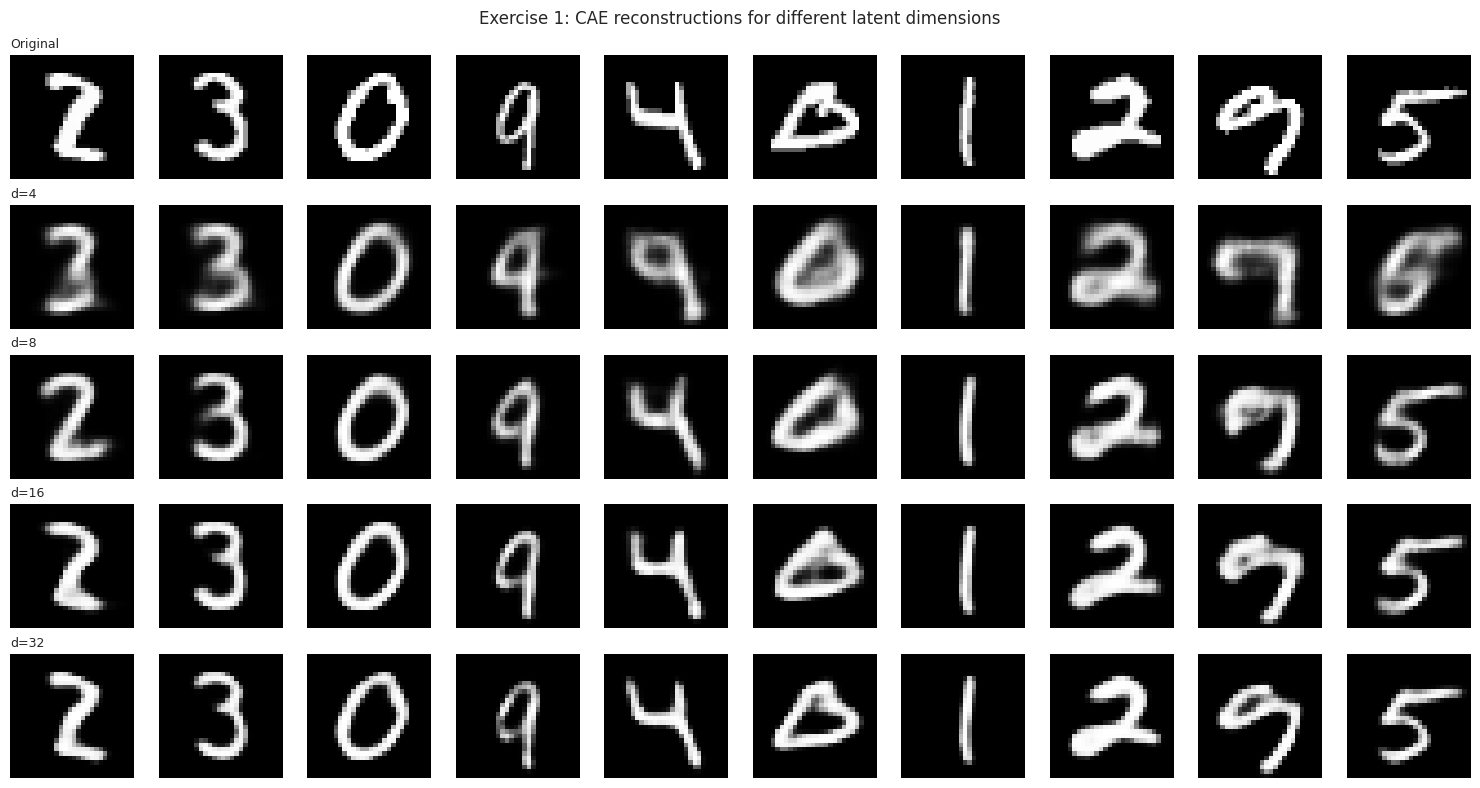
\includegraphics[width=0.4\textwidth]{add_plots/q1.png}
\end{center}
\begin{center}
\begin{tabular}{|c|c|c|c|}
\hline
Latent Dimension & MSE & SSIM & Parameters\\
\hline
4& 0.032648 & 0.650933& 65797\\
8  & 0.019939 & 0.784& 90889\\
16 & 0.010265 & 0.892806& 141073\\
32 & 0.006515 & 0.929655& 241441\\
\hline
\end{tabular}
\end{center}
\item \textbf{Compare Gaussian noise and salt-and-pepper noise using the
same denoising architecture.} 

\begin{center}
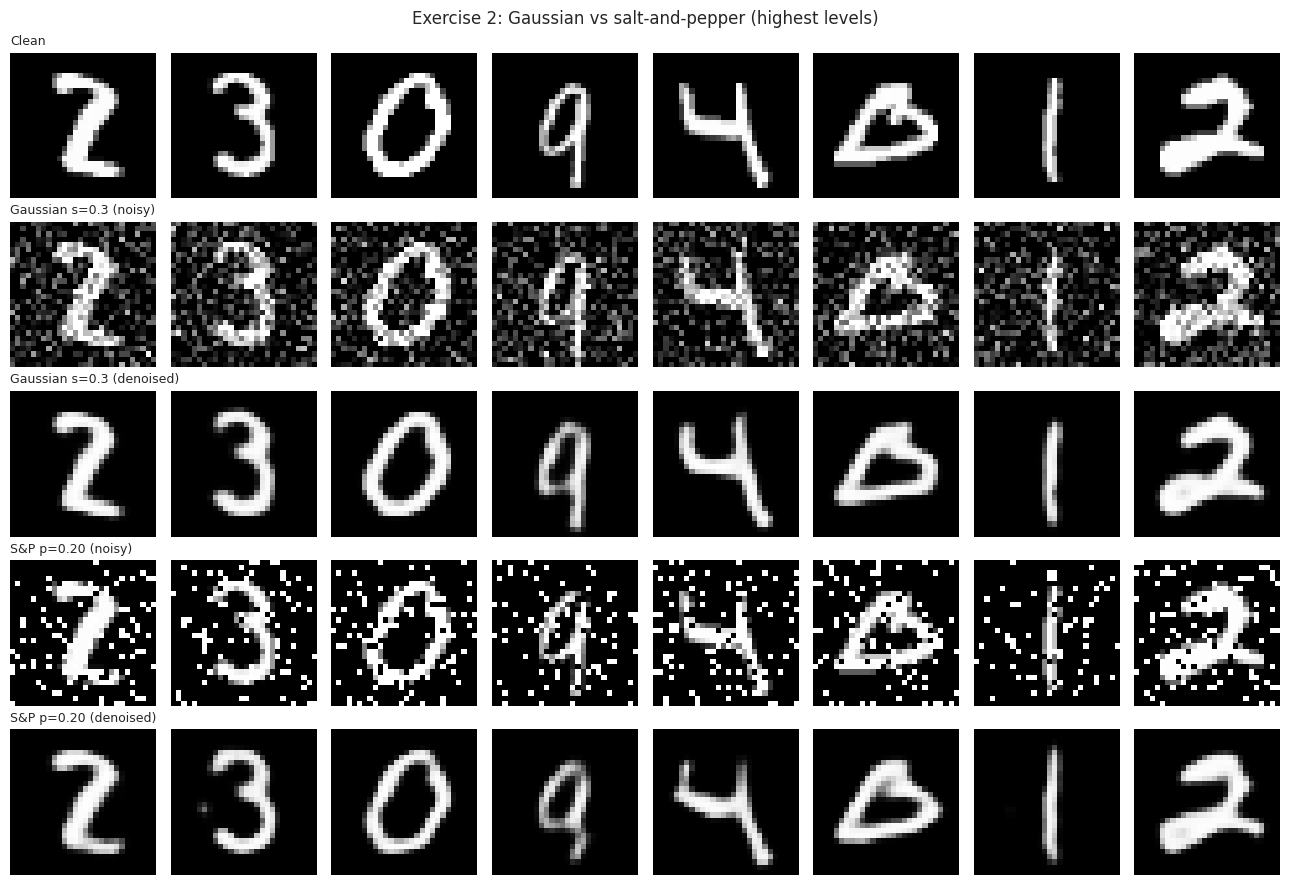
\includegraphics[width=0.4\textwidth]{add_plots/q2.png}
\end{center}

Inference: As noise level increases, denoised SSIM decreases gradually while MSE increases.  Salt-Pepper produces more corruption as seen from the high noisy MSE values but because of this it also gives the higher gain than gaussian noise. Overall, the model is able to reconstruct the images very well given any degree of noise level of gaussian and salt-pepper. 
\begin{table}[htbp]
\centering
\caption{Gaussian vs. Salt-and-Pepper Noise: Metrics Against Clean Images}
\begin{tabular}{l c c c c c c c}
\hline
\textbf{Noise Type} & \textbf{Level} & \textbf{Noisy MSE} & \textbf{Noisy SSIM} &
\textbf{Denoised MSE} & \textbf{Denoised MAE} & \textbf{Denoised SSIM} & \textbf{SSIM Gain} \\
\hline
Gaussian     & 0.10 & 0.0054 & 0.6932 & 0.0029 & 0.0164 & 0.9676 & 0.2744 \\
Gaussian     & 0.20 & 0.0212 & 0.6094 & 0.0042 & 0.0203 & 0.9501 & 0.3407 \\
Gaussian     & 0.30 & 0.0466 & 0.5248 & 0.0064 & 0.0256 & 0.9232 & 0.3984 \\
Salt-Pepper  & 0.05 & 0.0240 & 0.7193 & 0.0037 & 0.0182 & 0.9601 & 0.2408 \\
Salt-Pepper  & 0.10 & 0.0481 & 0.5932 & 0.0045 & 0.0203 & 0.9507 & 0.3574 \\
Salt-Pepper  & 0.20 & 0.0966 & 0.4608 & 0.0069 & 0.0265 & 0.9228 & 0.4620 \\
\hline
\end{tabular}
\end{table}

\item \textbf{Train the denoising autoencoder using two different noise
levels and compare SSIM.} 


\textbf{Inference :} Training only on $\sigma$=0.1\$ performs well on mild noise but degrades sharply on stronger unseen noise. Training on $\sigma$=0.3\$ generalizes much better across all test noise levels, maintaining SSIM above 0.92. Thus, training with stronger noise improves robustness to varying noise severity, at the cost of slightly worse performance on very mild noise. 

\begin{table}[htbp]
\centering
\caption{SSIM for Different Training and Testing Noise Levels}
\begin{tabular}{c c c c}
\hline
\textbf{Training $\sigma$} & \textbf{Test $\sigma=0.1$} & \textbf{Test $\sigma=0.2$} & \textbf{Test $\sigma=0.3$} \\
\hline
0.1 & 0.9678 & 0.8918 & 0.7172 \\
0.3 & 0.9546 & 0.9452 & 0.9233 \\
\hline
\end{tabular}
\end{table}

\begin{table}[htbp]
\centering
\caption{MSE for Different Training and Testing Noise Levels}
\begin{tabular}{c c c c}
\hline
\textbf{Training $\sigma$} & \textbf{Test $\sigma=0.1$} & \textbf{Test $\sigma=0.2$} & \textbf{Test $\sigma=0.3$} \\
\hline
0.1 & 0.00288 & 0.00465 & 0.00932 \\
0.3 & 0.00428 & 0.00491 & 0.00644 \\
\hline
\end{tabular}
\end{table}

\item \textbf{Replace the convolutional decoder with transposed
convolutions and compare the reconstructions.} 

\begin{center}
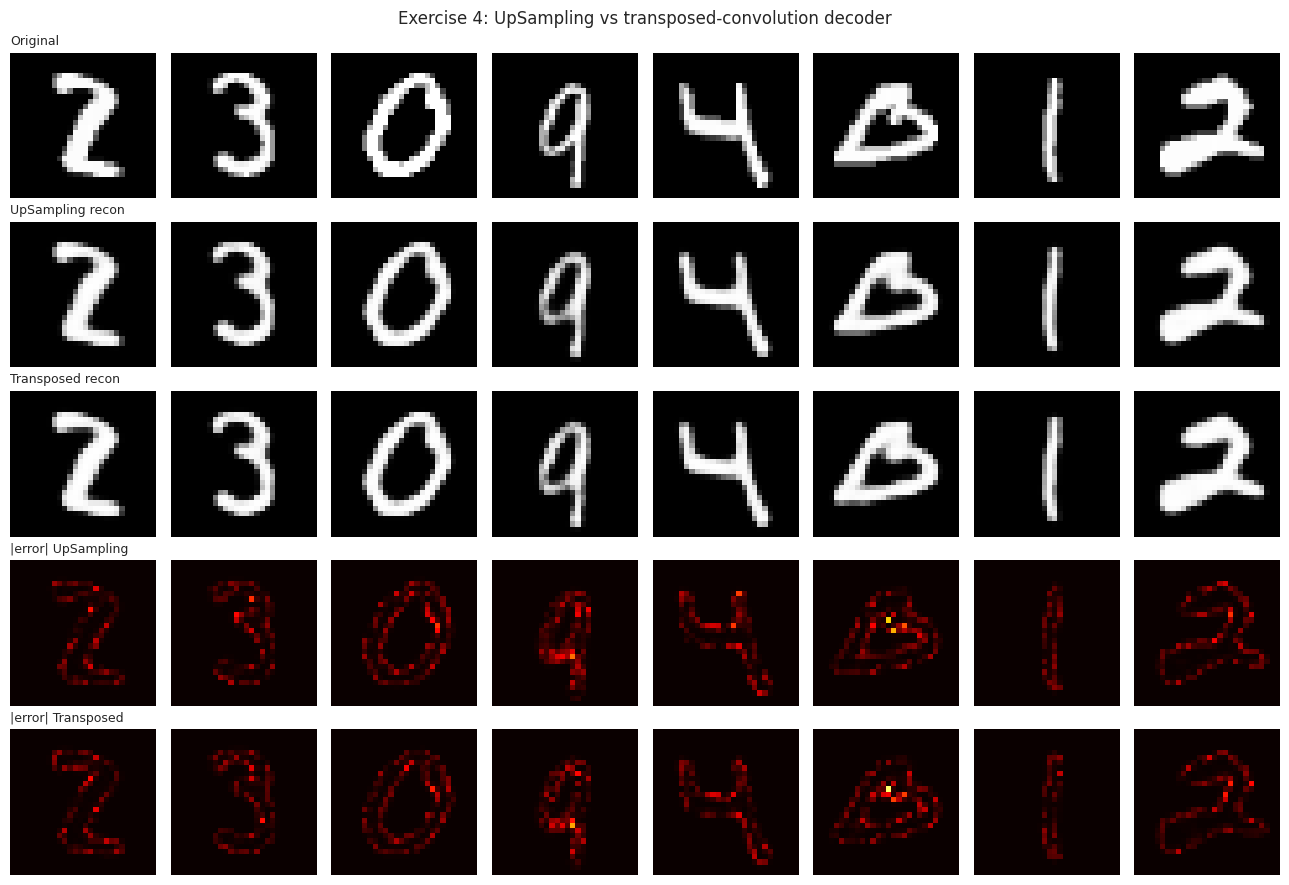
\includegraphics[width=0.4\textwidth]{add_plots/q4.png}
\end{center}

\textbf{Inference:} Conv2DTranspose achieves slightly lower MSE/MAE and higher SSIM, indicating marginally better reconstruction quality. Both architectures have the same number of parameters, while Conv2DTranspose is also faster (17.1 s vs. 19.0 s). 

\begin{table}[htbp]
\centering
\caption{Decoder Architecture Comparison}
\begin{tabular}{l c c c c c}
\hline
\textbf{Decoder} & \textbf{MSE} & \textbf{MAE} & \textbf{SSIM} & \textbf{Parameters} & \textbf{Time (s)} \\
\hline
UpSampling2D + Conv2D & 0.002413 & 0.014836 & 0.974513 & 74497 & 19.0 \\
Conv2DTranspose & 0.002292 & 0.014157 & 0.976977 & 74497 & 17.1 \\
\hline
\end{tabular}
\end{table}

\item \textbf{Implement a VAE with latent dimension 2 and 8 and compare
the latent representations.} 

\begin{center}
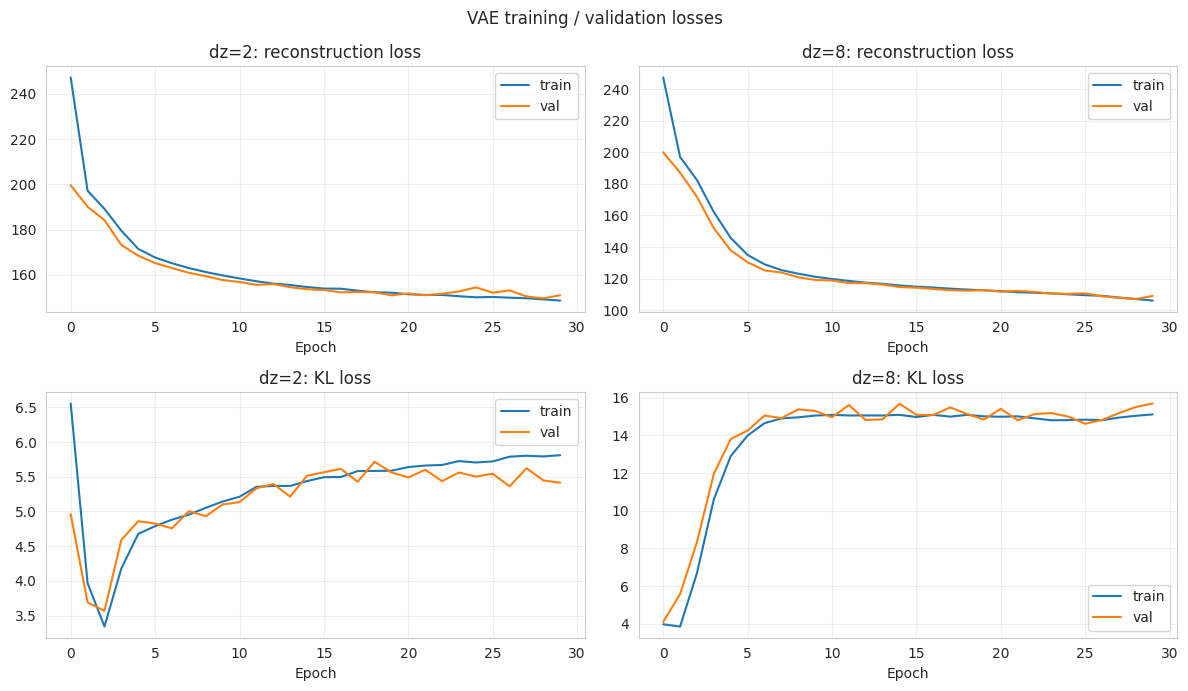
\includegraphics[width=0.4\textwidth]{add_plots/q5a.png}
\end{center}

\begin{center}
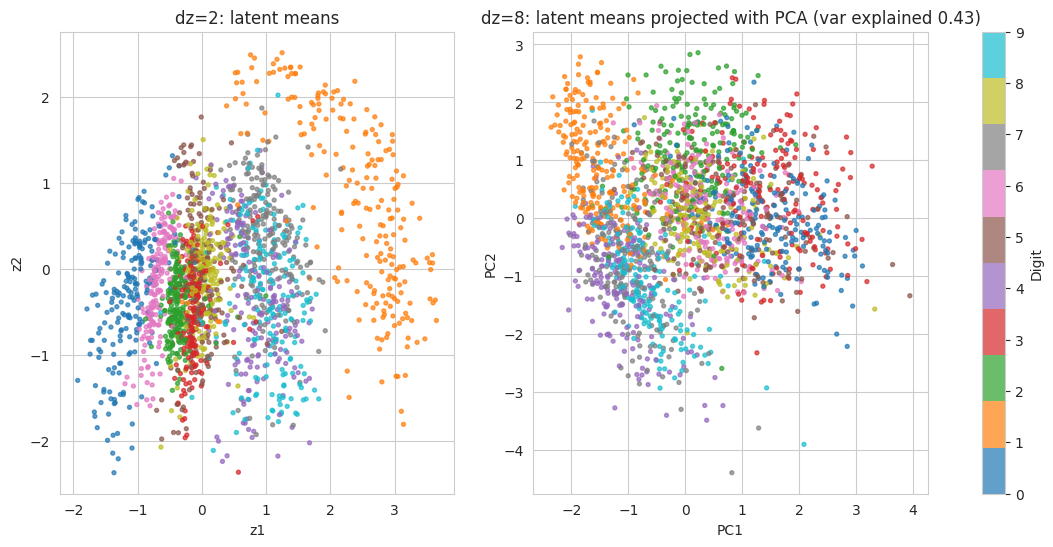
\includegraphics[width=0.4\textwidth]{add_plots/q5b.png}
\end{center}

\begin{center}
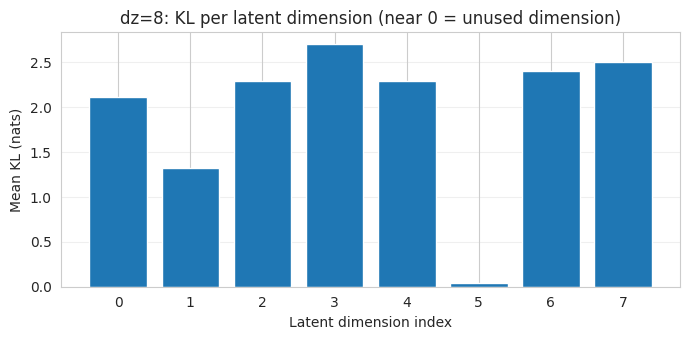
\includegraphics[width=0.4\textwidth]{add_plots/q5c.png}
\end{center}

\begin{center}
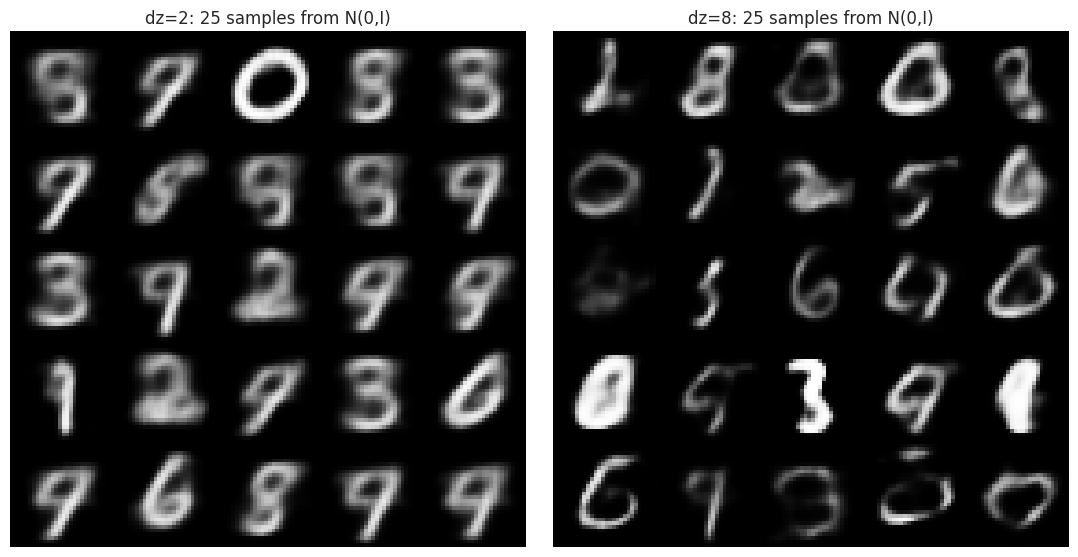
\includegraphics[width=0.4\textwidth]{add_plots/q5d.png}
\end{center}

Increasing the latent dimension from 2 to 8 substantially improves reconstruction, with SSIM increasing from \textbf{0.5064 to 0.7288} and MSE decreasing from \textbf{0.0439 to 0.0246}. The 8-dimensional VAE uses \textbf{7 active latent dimensions}, while one dimension has very low KL (\textbf{0.046}) and is effectively inactive. The additional capacity therefore captures more information about the MNIST images, with only a small increase in parameters and training time. 

\begin{table}[htbp]
\centering
\caption{VAE Comparison for Different Latent Dimensions}
\begin{tabular}{c c c c c c c c c c}
\hline
\textbf{Latent Dim.} & \textbf{Recon Loss} & \textbf{KL Loss} & \textbf{Total Loss} &
\textbf{MSE} & \textbf{MAE} & \textbf{SSIM} & \textbf{Parameters} &
\textbf{Active Dims.} & \textbf{Time (s)} \\
\hline
2 & 149.7670 & 5.4152 & 155.1822 & 0.0439 & 0.1049 & 0.5064 & 141189 & 2 & 28.5 \\
8 & 105.9217 & 15.6893 & 121.6110 & 0.0246 & 0.0639 & 0.7288 & 141489 & 7 & 29.5 \\
\hline
\end{tabular}
\end{table}

\begin{table}[htbp]
\centering
\caption{KL Divergence per Latent Dimension for $d_z=8$}
\begin{tabular}{c c c c c c c c}
\hline
\textbf{Dim. 1} & \textbf{Dim. 2} & \textbf{Dim. 3} & \textbf{Dim. 4} &
\textbf{Dim. 5} & \textbf{Dim. 6} & \textbf{Dim. 7} & \textbf{Dim. 8} \\
\hline
2.119 & 1.323 & 2.293 & 2.701 & 2.295 & 0.046 & 2.405 & 2.506 \\
\hline
\end{tabular}
\end{table}

\item \textbf{Investigate the effect of increasing the KL-loss
contribution.} 

\begin{center}
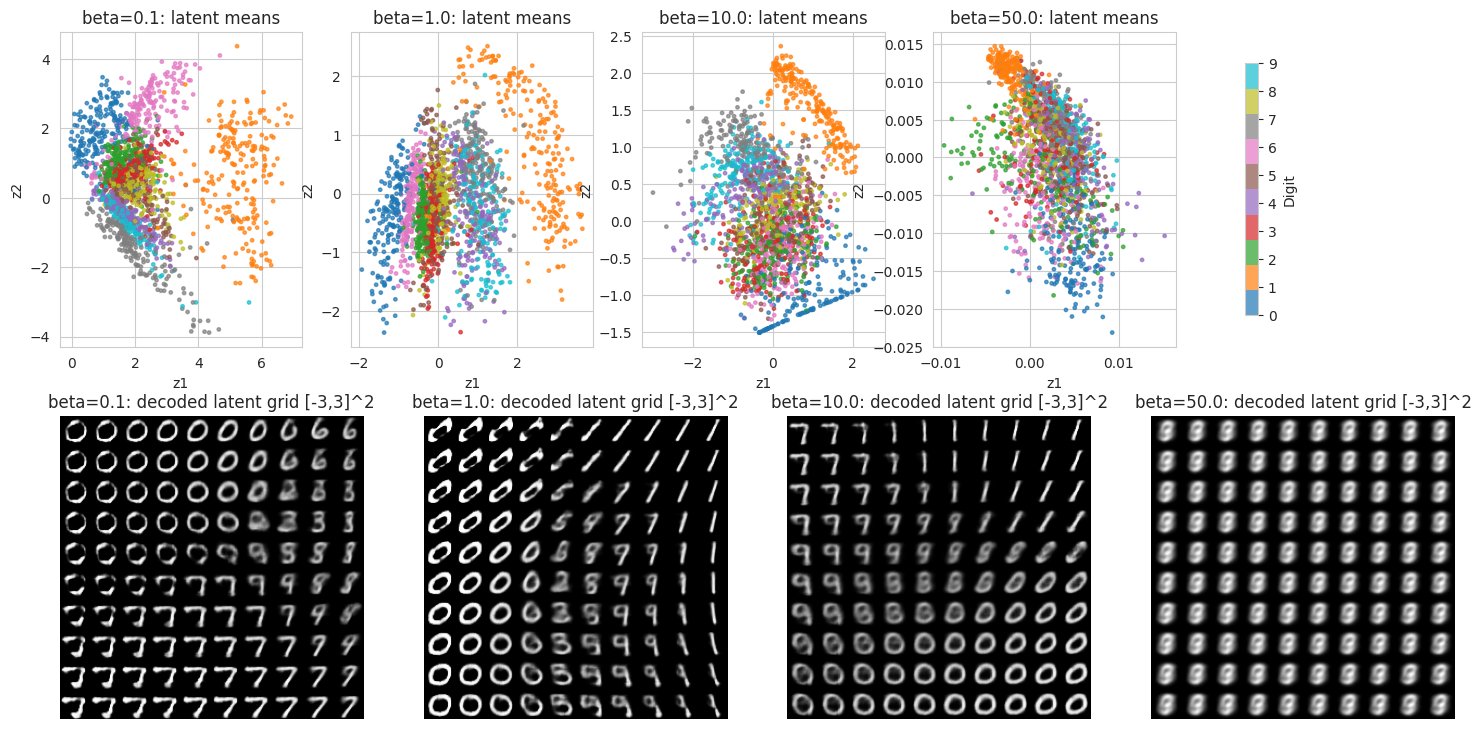
\includegraphics[width=0.4\textwidth]{add_plots/q6.png}
\end{center}

\textbf{Inference:} Increasing $\beta$ forces the latent distribution closer to the prior, reducing KL divergence and eventually causing \textbf{latent collapse} (0 active dimensions at $\beta$  = 50). Reconstruction quality is relatively stable for $\beta$  = 1 , but deteriorates sharply for larger $\beta$, with SSIM falling from \textbf{0.5064 to 0.1788}. Thus, a moderate $\beta$  provides a better balance between latent regularization and reconstruction quality. 

\begin{table}[htbp]
\centering
\caption{Effect of $\beta$ on VAE Performance}
\begin{tabular}{c c c c c c}
\hline
\textbf{$\beta$} & \textbf{Recon Loss} & \textbf{KL Loss} & \textbf{MSE} &
\textbf{SSIM} & \textbf{Active Dims.} \\
\hline
0.1  & 149.0002 & 12.0877 & 0.0439 & 0.5043 & 2 \\
1.0  & 149.7670 & 5.4152  & 0.0439 & 0.5064 & 2 \\
10.0 & 164.4278 & 1.7802  & 0.0504 & 0.3969 & 2 \\
50.0 & 203.9250 & 0.0001  & 0.0667 & 0.1788 & 0 \\
\hline
\end{tabular}
\end{table}

\item \textbf{Generate a larger grid of VAE samples and discuss
diversity.} 

\begin{center}
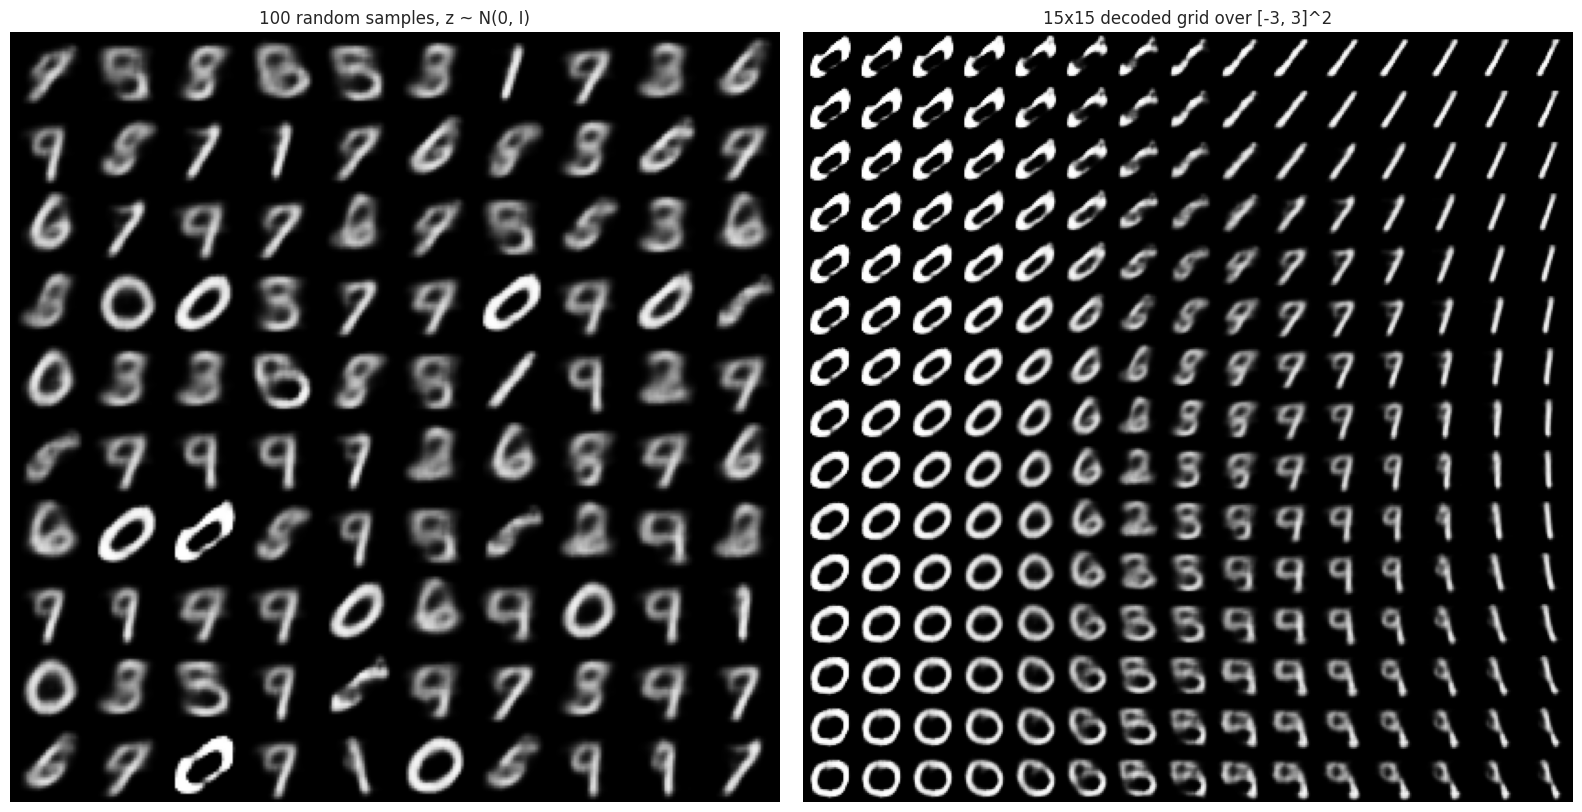
\includegraphics[width=0.4\textwidth]{add_plots/q7a.png}
\end{center}

\begin{center}
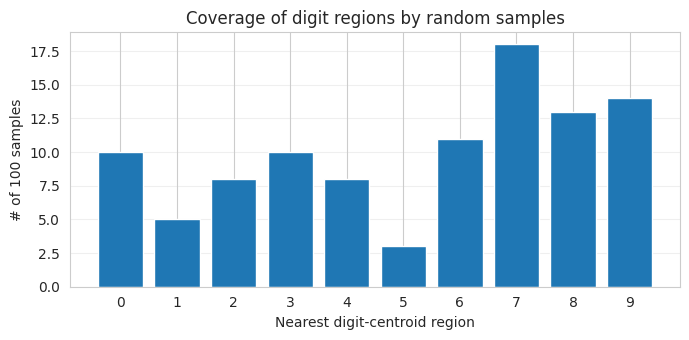
\includegraphics[width=0.4\textwidth]{add_plots/q7b.png}
\end{center}

\item 
Inference:
\textbf{The 100 random samples demonstrate that the 2D VAE can generate diverse MNIST-like digits from random latent vectors, covering multiple digit classes and styles. The samples are not equally distributed across all digit regions, with digit 7 being the most represented and digit 5 the least represented, indicating uneven coverage of the latent space. The smooth transitions in the 15×15 latent grid further show that nearby latent points produce gradually changing digit structures.}


 

\item \textbf{Select two digit regions in the latent space and perform
interpolation.}

\begin{center}
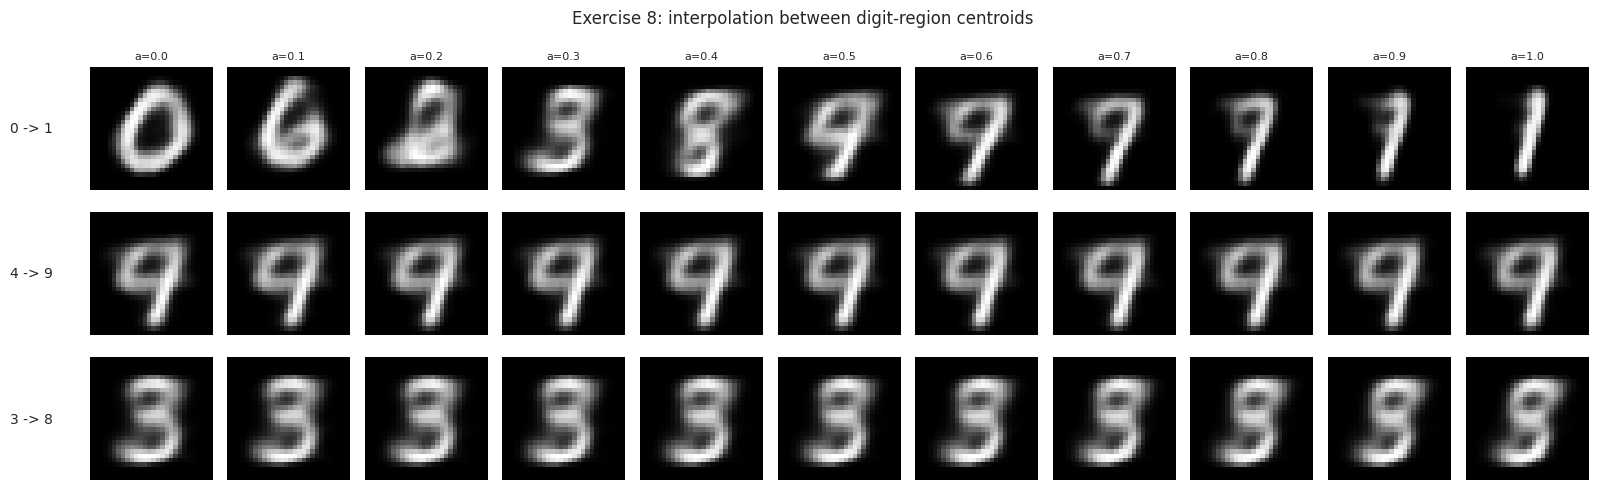
\includegraphics[width=0.4\textwidth]{add_plots/q8a.png}
\end{center}

\begin{center}
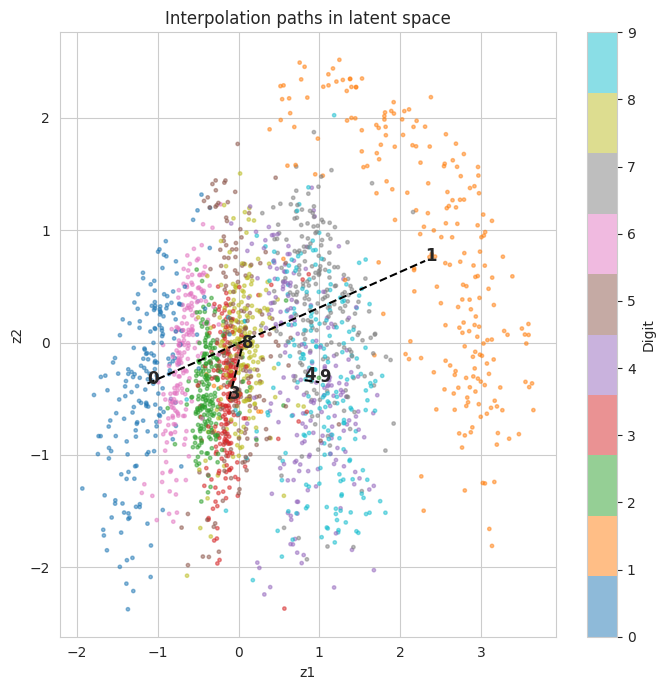
\includegraphics[width=0.4\textwidth]{add_plots/q8b.png}
\end{center}

\textbf{Inference:} Linear interpolation between digit-region centroids produces smooth transitions between latent representations, with the generated images gradually changing from one digit to another. This indicates that the VAE has learned a continuous and structured latent space where nearby regions correspond to related digit representations. However because of overlaps in as seen earlier, the 4 > 9 row shows the first image(as well as the rest) as a 9, inidcating significant overlaps betweent the 4 and 9 clusters in latent space.

\end{enumerate}

%%%%%%%%%%%%%%%%%%%%%%%%%%%%%%%%%%%%%%%%%%%%%%%%%%%%%%%%%%%%
\section*{31. Expected Outcome}

At the end of the experiment, students should be able to demonstrate the
complete image-representation and reconstruction pipeline:

\[
\boxed{
\text{Image}
\rightarrow
\text{Encoder}
\rightarrow
\text{Latent Representation}
\rightarrow
\text{Decoder}
\rightarrow
\text{Reconstructed Image}
}
\]

They should also demonstrate denoising:

\[
\boxed{
\text{Clean Image}
\rightarrow
\text{Noise}
\rightarrow
\text{Denoising Autoencoder}
\rightarrow
\text{Recovered Image}
}
\]

and variational generation:

\[
\boxed{
\text{Image}
\rightarrow
(\mu,\sigma)
\rightarrow
z
\rightarrow
\text{Decoder}
\rightarrow
\text{Generated/Reconstructed Image}
}
\]

\textbf{Key results from this run:}

\begin{itemize}
\item FC Autoencoder: fast to train, but visibly blurry, thicker-stroked
reconstructions (SSIM 0.7621) due to loss of spatial structure through
flattening.
\item Convolutional AE: sharp, high-fidelity reconstructions (SSIM 0.9746)
leveraging spatial locality, using only 35\% as many parameters as the FC
model.
\item Denoising CAE: effectively removes Gaussian noise and recovers digit
structure across all tested noise levels (SSIM 0.89--0.96 for
$\sigma=0.1$--$0.3$).
\item VAE: enables smooth latent-space interpolation (Section 21) and
generation, but with a 2D latent space and a 10-class dataset, the
learned latent space under-separates most digit classes (Section 19),
which in turn produces generated samples with visibly limited diversity
(Section 20) and the weakest reconstruction metrics of the four models
(SSIM 0.4865).
\end{itemize}

The final report contains both quantitative evaluation and visual
analysis. All numerical values above were obtained from the student's own
notebook execution.

%%%%%%%%%%%%%%%%%%%%%%%%%%%%%%%%%%%%%%%%%%%%%%%%%%%%%%%%%%%%
\section*{32. References}

\begin{enumerate}
\item Ian Goodfellow, Yoshua Bengio and Aaron Courville,
\emph{Deep Learning}, MIT Press, 2016.

\item Diederik P. Kingma and Max Welling,
``Auto-Encoding Variational Bayes,'' ICLR, 2014.

\item Pascal Vincent et al.,
``Stacked Denoising Autoencoders: Learning Useful Representations in a Deep
Network with a Local Denoising Criterion,'' Journal of Machine Learning
Research, 2010.

\item Yann LeCun, Corinna Cortes and Christopher J. C. Burges,
``MNIST Handwritten Digit Database.''

\item TensorFlow Documentation:
\url{https://www.tensorflow.org}

\item Keras Documentation:
\url{https://keras.io}

\item scikit-image Documentation:
\url{https://scikit-image.org}
\end{enumerate}

\end{document}